\documentclass[aps,prapplied,reprint,superscriptaddress]{revtex4-2}

\usepackage{amsmath,amssymb}
\usepackage{graphicx}
\usepackage{booktabs}
\usepackage{tabularx}
\usepackage{array}
\usepackage{multirow}
\usepackage{enumitem}
\usepackage{placeins}
\usepackage{xcolor}
\usepackage{url}

\graphicspath{{figures/}}

\begin{document}

\title{Memory Physics, Finite Capacity, and Topology in Heterogeneous Quantum Networks}

\author{David Vesterlund}
\affiliation{Vesterlund Ventures, WestQuant Open}
\email{david@vesterlundventures.se}

\date{8 October 2026}

\thanks{ORCID: 0009-0000-6455-1141}

\begin{abstract}
Quantum-network capacity planning couples memory physics, finite storage, topology, and traffic. We study these interactions using a discrete-event simulator with six representative memory profiles. A memory--topology atlas contains 9{,}360 completed runs, complemented by 8{,}730 confirmatory runs and an extended per-node memory-budget sweep. We distinguish a threshold relative to the best performance observed on a finite grid from a physical saturation limit. Among 840 reported threshold estimates, 22.3\% reach 95\% of the observed maximum by four slots per node, while 35.5\% first reach it at the upper grid boundary of 64 slots. Four tested scalar reductions do not provide a topology-independent collapse; the best pooled quadratic fit explains 37.9\% of response variance. The retrieval-window parameter $\chi_r = \tau_r\, p_{\rm gen} / t_{\rm attempt}$ provides an interpretable descriptor, but an independent-channel approximation does not establish a network memory-sizing law. In 5{,}310 heterogeneous-placement runs, hub and betweenness-based placement outperform peripheral placement in aggregate, with topology-specific exceptions. Coupling assumptions change absolute performance while preserving the aggregate strategy ordering. Harmonized model comparisons provide limited robustness evidence, not independent native-protocol validation. The results support model-specific capacity and placement analysis with explicit metric definitions, finite-grid limitations, and interface assumptions.
\end{abstract}

\maketitle

\begin{figure*}[t]
\centering
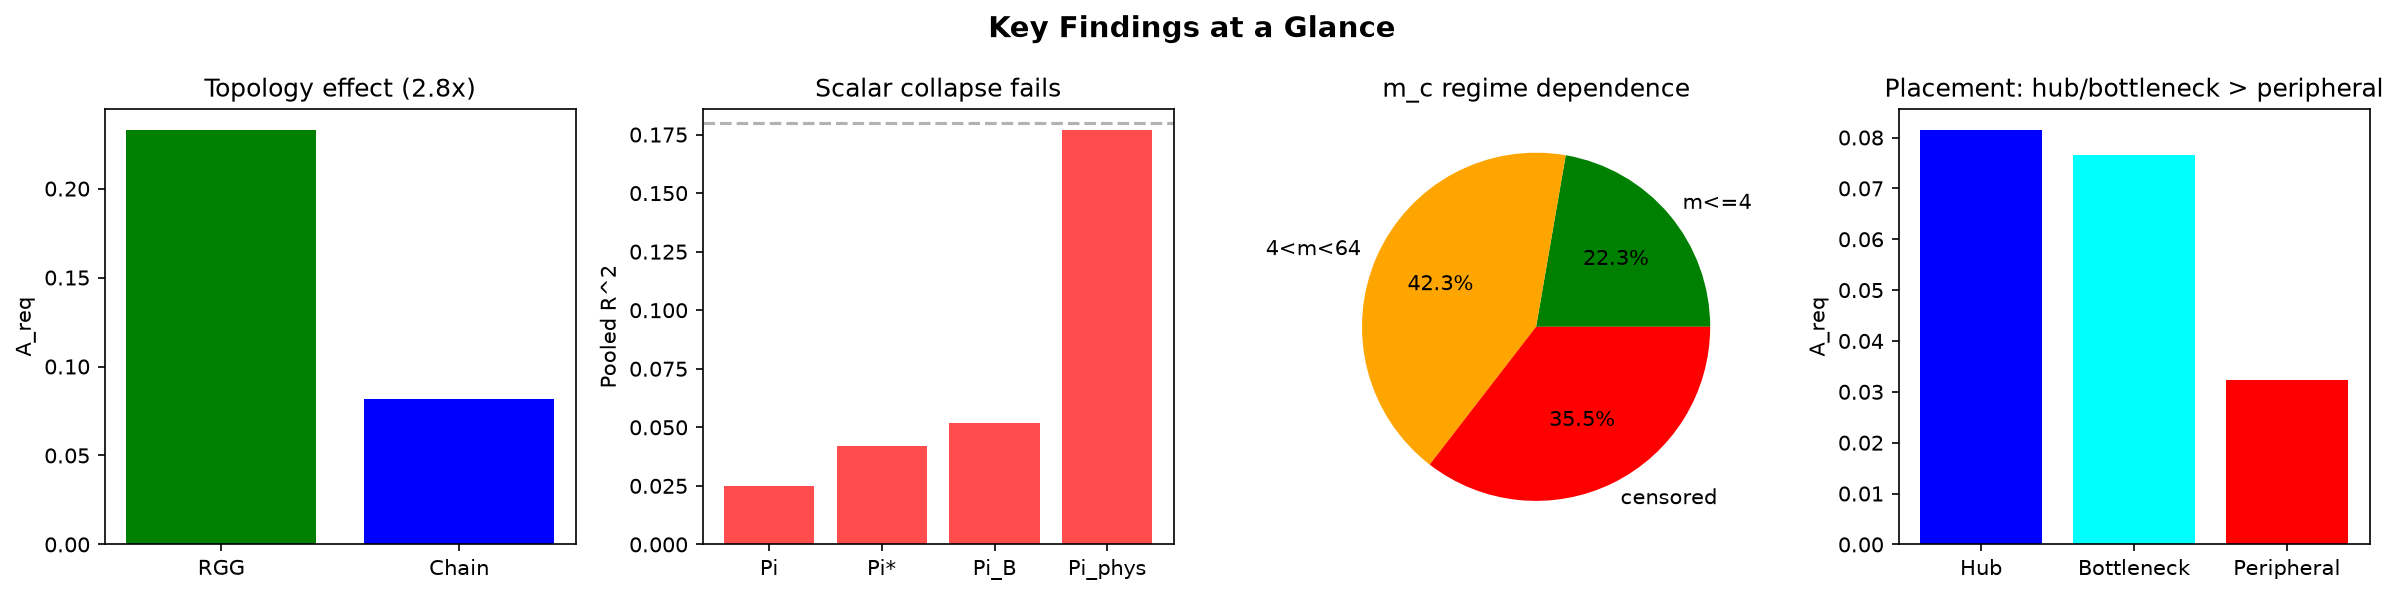
\includegraphics[width=0.98\textwidth]{fig_key_findings.png}
\caption{Key findings at a glance. The retrieval-window parameter $\chi_r = \tau_r\, p_{\rm gen} / t_{\rm attempt}$ (where $\tau_r$ is the retrieval decay time, not $T_2$) provides an interpretable descriptor but does not establish a universal memory-sizing law; the 95\%-of-observed-maximum memory threshold is strongly regime-dependent with 35.5\% of regimes as boundary cases at $m=64$; and hub/bottleneck placement outperforms peripheral placement in aggregate under the tested heterogeneous configurations.}
\label{fig:key_findings}
\end{figure*}

\noindent\textbf{Keywords:} quantum networks, quantum memory, discrete-event simulation, finite capacity, heterogeneous placement, reproducibility

\section{Introduction}

Quantum networks promise distributed quantum computation, secure communication, and distributed sensing~\cite{wehner2018quantum}. A central engineering question is not simply \textit{which memory technology is best}, but rather: \textit{how do physical memory properties, finite capacity, network position, topology, and offered load jointly determine useful end-to-end entanglement?} This question couples device-level physics (coherence time, retrieval efficiency, readout fidelity, physical interfaces) to network-level structure (topology, routing, contention), and its answer determines hardware--network co-design rules for heterogeneous quantum networks. Figure~\ref{fig:key_findings} summarizes the key findings of this study.

Existing analytical results characterize scaling and rate--memory trade-offs for specific repeater architectures, often homogeneous chains with prescribed memory models~\cite{razavi2009quantum,sangouard2011quantum,chehimi2023scaling}. Simulation frameworks such as SeQUeNCe~\cite{wu2021sequence}, NetSquid~\cite{coopmans2021netsquid}, and QuISP~\cite{satoh2022quisp} enable more detailed studies, while recent cross-validation work shows that simulator assumptions can materially affect timing even when fidelity agrees~\cite{vittal2025cross}. Recent work on heterogeneous link architectures~\cite{sharma2024heterogeneous} and hybrid repeater designs~\cite{van2025hybrid,liu2025hybrid} motivates the question of whether conclusions derived from homogeneous models transfer to heterogeneous hardware.

Simulation-based network-design conclusions are valuable only if they are not artifacts of a single implementation. We therefore supplement the component-level analytical validation with a harmonized cross-implementation robustness check (Sec.~\ref{sec:cross_impl}), in which selected conclusions are re-evaluated through harmonized implementations executed on the SeQUeNCe and SimQN event frameworks. The purpose is to test whether selected structural conclusions survive an independent implementation/event-framework pathway, not to establish universal simulator invariance. A companion reliability study reports the full simulator-invariance methodology.

This paper addresses four research questions:

\begin{description}[leftmargin=2em]
\item[\textbf{RQ-A1}] Which memory- and network-level parameters limit end-to-end entanglement delivery?
\item[\textbf{RQ-A2}] How does performance vary across representative memory profiles and topologies?
\item[\textbf{RQ-A3}] Does a universal scaling law for memory sufficiency exist?
\item[\textbf{RQ-A4}] How does heterogeneous memory hardware affect conclusions?
\end{description}

Our central thesis is:
\begin{quote}
\textit{Within the investigated operating regimes, the per-node memory-budget threshold $m_c$ is strongly regime-dependent and does not collapse to a topology-independent scalar. The retrieval-window parameter $\chi_r = \tau_r\, p_{\rm gen} / t_{\rm attempt}$ (where $\tau_r$ is the retrieval decay time, not the coherence time $T_2$) provides an interpretable physical descriptor, but an independent-channel approximation does not establish a network memory-sizing law. Conclusions about heterogeneous memory deployment additionally require explicit interface modeling.}
\end{quote}

We do \textbf{not} claim that no universal scaling law can exist, that one memory technology is universally superior, or that the observed saturation behavior constitutes a fundamental physical law. Our claims are restricted to the tested models, parameter ranges, and operating regimes.

\textbf{The retrieval-window descriptor.} A physical timescale descriptor used in this paper is the coincidence-window parameter
\begin{equation}
\chi_r \;=\; \frac{\tau_r\, p_{\rm gen}}{t_{\rm attempt}} \,,
\label{eq:chi}
\end{equation}
where $\tau_r$ is the retrieval decay time (not the coherence time $T_2$), $p_{\rm gen}$ is the per-attempt link generation success probability, and $t_{\rm attempt}$ is the link attempt interval. The parameter $\chi_r$ counts the expected number of successful link generations within one memory lifetime and separates two operating regimes:

\begin{description}[leftmargin=2em]
\item[\textbf{Coincidence-limited} ($\chi_r \ll 1$):] Link success within the retrieval lifetime is rare. The single-link memory threshold is
\begin{equation}
m \;\approx\; \frac{\ln(1-\alpha)}{\ln(1 - p_w)} \,, \qquad p_w = 1 - (1 - p_{\rm gen})^{\tau_r/t_{\rm attempt}} \,,
\label{eq:chi_coincidence}
\end{equation}
where $p_w$ is the probability of at least one link success during the memory lifetime and $\alpha$ is the target fraction of peak performance.
\item[\textbf{Queue-limited} ($\chi_r \gg 1$):] Many link successes occur within the retrieval lifetime, and memory demand is governed by Little's law ($m \propto$ load $\times$ wait time) rather than by coincidence probability.
\end{description}

For multi-hop paths of length $h$, the path-success probability is $p_{\rm path} = p_w^{\,h}$ (all links must succeed), so the memory threshold scales with hop length. Table~\ref{tab:chi_regimes} maps the four primary memory profiles to their $\chi_r$ values and regimes.

\begin{table}[htbp]
\centering
\caption{Regime map for the four primary memory profiles at atlas parameters ($p_{\rm gen}=0.005$, $t_{\rm attempt}=10^{-3}$~s). $\chi_r = \tau_r \cdot p_{\rm gen} / t_{\rm attempt}$.}
\label{tab:chi_regimes}
\begin{tabular}{lrl}
\toprule
Profile & $\chi_r$ & Regime \\
\midrule
Trapped Ion & 50 & Queue-limited ($\chi_r \gg 1$) \\
Neutral Atom & 0.5 & Transitional ($\chi_r \sim 1$) \\
Diamond (Electron) & 0.22 & Coincidence-limited ($\chi_r \ll 1$) \\
AFC & 0.025 & Coincidence-limited ($\chi_r \ll 1$) \\
\bottomrule
\end{tabular}
\end{table}

The retrieval-window descriptor $\chi_r$ provides a physical interpretation of the regime-dependent $m_c$ distribution (Sec.~\ref{sec:chi_law}). No predictive accuracy or invariance rate is asserted for $\chi_r$ in this revision; the independent-channel approximation is an illustrative reference, not a validated network memory-sizing law.

\section{Related Work}

\subsection{Quantum Repeater Scaling}

Scaling behavior for quantum repeaters has been analyzed under a range of homogeneous-chain assumptions. Razavi, Piani, and L{\"u}tkenhaus~\cite{razavi2009quantum} showed that finite memory coherence can change favorable polynomial distance scaling into an exponential degradation in $\sqrt{L}$ in their optimized repeater model. More recent work studies exact rate analysis with imperfect memories~\cite{kamin2023exact} and joint optimization of repeater count, spacing, and distillation under rate and fidelity constraints~\cite{chehimi2023scaling}. These results provide important benchmarks, but they do not directly address the cross-product of heterogeneous memory profiles and network topology studied here.

\subsection{Topology and Entanglement Distribution}

The impact of network topology on entanglement distribution has been studied by several groups. Ooi, Sutcliffe, and Beghelli~\cite{alhejji2026topology} identified four topology-dependent performance regimes across 81 real topologies. Ozaydin et al.~\cite{ozaydin2025multiring} developed optimal algorithms for multi-ring topologies. Vardoyan et al.~\cite{amin2023capacity} derived end-to-end capacity bounds via flow maximization. Pirandola~\cite{pirandola2019endtoend} derived end-to-end capacity bounds for quantum networks. Takeoka et al.~\cite{takeoka2016rateloss} established the fundamental rate-loss tradeoff for optical quantum communication, constraining the achievable rates that any network design must respect. Vasantam and Towsley~\cite{vardoyan2021maxweight} analyzed the stability of quantum networks with max-weight scheduling, providing a queueing-theoretic foundation for resource contention analysis. These studies focus on routing, capacity, and scheduling rather than memory-physics interactions.

\subsection{Heterogeneous Quantum Networks}

Recent work has begun exploring heterogeneous hardware. Soon et al.~\cite{sharma2024heterogeneous} demonstrated that mixed link architectures work without significant rate loss using QuISP. Van Loock et al.~\cite{van2025hybrid} and Liu et al.~\cite{liu2025hybrid} proposed hybrid repeater architectures combining trapped ions, neutral atoms, and AFC memories. These studies motivate, but do not replace, a controlled comparison of representative memory profiles across multiple topology classes and placement rules.

\subsection{Resource Placement}

Repeater and memory placement has been formulated as an optimization problem. Pouryousef et al.~\cite{pouryousef2024resource} developed a network-planning framework that allocates repeaters and memories while accounting for rate, fidelity, multiplexing, and coherence. Sripotchanart et al.~\cite{sripotchanart2024twostep} proposed a scalable two-step linear-programming approach for repeater placement, while Islam and Arslan~\cite{islam2023scalable} developed fast heuristic deployment models. Our focus differs: we hold the network-planning objective fixed and study how heterogeneous memory quality, finite capacity, topology, and interface assumptions interact.

\subsection{Simulator Validation}

Cross-validation of quantum network simulators is an emerging concern. Chung et al.~\cite{vittal2025cross} cross-validated QuISP and SeQUeNCe, finding that different simulator assumptions can produce different timing results even when fidelity results agree after harmonization. This motivates careful validation of any single-simulator study. The present work supplements its component-level analytical validation with a harmonized cross-implementation robustness study (Sec.~\ref{sec:cross_impl}). We emphasize that this cross-implementation check does not yet use native SeQUeNCe or SimQN protocols, does not include NetSquid or QuISP, and that the SeQUeNCe and SimQN adapters share a common harmonized model. The purpose is therefore to test whether selected conclusions survive an independent implementation/event-framework pathway, not to establish universal simulator invariance.

\section{Quantum Memory and Network Model}
\label{sec:model}

\subsection{Representative Memory Profiles}

We model six representative quantum-memory profiles using literature-informed parameter bundles (Table~\ref{tab:memory}):

\begin{table}[htbp]
\centering
\caption{Representative memory-profile parameters. $T_1$ and $T_2$ are in seconds, $\eta_r$ is retrieval efficiency at $t=0$, $\tau_r$ is the retrieval decay time (s), and $F_{ro}$ is readout fidelity. Provenance and source citations are provided in Supplemental Table~S1~\cite{langer2005long,wang2014high,wang2024fine,hosseini2006gem,wang2018eit,balasubramanian2009ultralong,steiner2010universal,bradley2022robust,maurer2012room,rielandner2021storage,laplane2017multimode,reagor2016quantum}.}
\label{tab:memory}
\begin{tabular}{lrrrrr}
\toprule
Profile & $T_1$ (s) & $T_2$ (s) & $\eta_r$ & $\tau_r$ (s) & $F_{ro}$ \\
\midrule
Trapped Ion & 100 & 10.0 & 0.90 & 10.0 & 0.999 \\
Neutral Atom & 1.0 & 0.1 & 0.80 & 0.5 & 0.99 \\
Diamond (Electron) & 1.0 & 0.044 & 0.70 & 0.1 & 0.95 \\
Diamond (Nuclear) & 100 & 1.3 & 0.50 & 1.0 & 0.95 \\
AFC & 10 & 0.005 & 0.50 & 0.01 & 0.99 \\
Superconducting & 0.001 & 0.0001 & 0.95 & 0.001 & 0.999 \\
\bottomrule
\end{tabular}
\end{table}

These profiles are \textit{representative bundles}, not complete device-level hardware comparisons. Some bundles combine characteristic values reported for related implementations within a memory platform; Supplemental Table~S1 therefore labels each numerical entry as MEASURED, DERIVED, or ASSUMED. The simulated budget $m$ is an abstract number of independently usable memory slots per node and is not identified with an experimentally reported multimode capacity.

\subsection{Network Topologies}

We study nine topology classes: chain, star, random geometric graph (RGG), Waxman, hierarchical, lattice, scale-free, binary tree, and ring. Topologies are generated with controlled parameters (node count, edge density, geographic extent).

\subsection{Simulator}

Our discrete-event simulator models:
\begin{itemize}[leftmargin=2em]
\item Per-node memory capacity via a \textit{placement} dictionary
\item Homogeneous or heterogeneous memory profiles
\item Homogeneous or heterogeneous decoherence models
\item Depolarizing, dephasing, or amplitude-damping noise
\item Serial or parallel link generation
\item Entanglement swapping with configurable success probability
\item Retrieval efficiency and readout fidelity
\item Deadline-based service qualification
\item Poisson request arrivals with optional traffic matrices
\item Warmup and censoring to reduce transient artifacts
\end{itemize}

Table~\ref{tab:sim_params} lists the default simulator parameters.

\begin{table}[htbp]
\centering
\caption{Simulator parameters used throughout the paper unless otherwise stated.}
\label{tab:sim_params}
\resizebox{\linewidth}{!}{%
\begin{tabular}{lll}
\toprule
Parameter & Value & Description \\
\midrule
$p_{\rm gen}$ & 0.005 & Link generation success probability \\
$t_{\rm attempt}$ & $10^{-3}$ s & Link attempt interval \\
Deadline & 1.0 s & Request deadline \\
$F_{\rm min}$ & 0.5 & Minimum fidelity for qualification \\
$p_{\rm swap}$ & 0.98 & Entanglement swap success probability \\
$F_{\rm initial}$ & 0.9 & Initial link fidelity \\
$T_{\rm obs}$ & 200 s & Simulation observation time \\
Warmup & First 10\% of requests & Warmup period \\
$n_{\rm requests}$ & 100 & Requests per simulation \\
\bottomrule
\end{tabular}%
}
\end{table}

Noise levels are defined for the sensitivity analysis (Sec.~\ref{sec:sensitivity}) as: \textbf{low} = 0.1$\times$ baseline depolarizing rate, \textbf{medium} = 1.0$\times$ baseline, \textbf{high} = 10$\times$ baseline. The baseline depolarizing rate is derived from the memory profile's $T_2$. In the atlas and confirmatory experiments, noise is not independently varied; the depolarizing rate is fixed by each profile's $T_2$.

\textbf{Run-length caveat:} With $n_{\rm requests} = 100$ and the highest traffic level $\lambda = 50$, the observation window covers approximately $100/50 = 2$~s of simulated time. This is short relative to the $T_{\rm obs} = 200$~s parameter and may not reach full stationarity for queueing dynamics at high load. The warmup period (first 10\% of requests) partially mitigates transient effects, but the high-traffic results should be interpreted with the caveat that the system may not have fully reached steady state.

The primary performance metric is $A_{\rm req}$: the fraction of \textit{effective incoming requests} (excluding warmup, censored, and no-path requests) that are completed within deadline. A companion metric $A_{\rm qual}$ additionally requires the final fidelity to exceed $F_{\rm min}$. Quality-qualified throughput showed stronger ordinal agreement across the tested harmonized implementations than completion-only throughput. Because request-processing and denominator conventions were not fully identical across implementations, we treat this as a robustness observation rather than as a general superiority claim for either metric. All confidence intervals reported in this paper are 95\% bootstrap intervals (10{,}000 resamples, percentile method) computed across seeds unless otherwise stated.

\textbf{Definition of $m$:} Throughout this paper, $m$ denotes the \textit{per-node memory budget}: every node is assigned $m$ memory slots. This definition is used consistently in the atlas, the confirmatory replication, and the $m_c$ audit.

\subsection{Mathematical Model}
\label{sec:math_model}

The simulator's quantum-state and noise models are defined as follows.

\textbf{Werner-state parameterization.} Each entangled link is represented as a Werner state with fidelity $F$ to the target Bell state $|\Phi^+\rangle$:
\begin{equation}
\rho = F\,|\Phi^+\rangle\langle\Phi^+| + \frac{1-F}{3}\sum_{i}|\Psi_i\rangle\langle\Psi_i|,
\end{equation}
where $\{|\Psi_i\rangle\} = \{|\Phi^-\rangle, |\Psi^+\rangle, |\Psi^-\rangle\}$ are the other three Bell states. The Werner state is entangled iff $F > 0.5$.

\textbf{Decoherence channels.} During memory storage, the depolarizing channel drives $F$ toward the completely mixed value $F = 0.25$:
\begin{equation}
F(t) = 0.25 + (F_0 - 0.25)\,\exp(-\Gamma\, t),
\end{equation}
where $\Gamma$ is the depolarizing rate derived from the memory profile's $T_2$. The simulator also supports pure dephasing and amplitude-damping channels; in the atlas and confirmatory experiments, the depolarizing channel is used with $\Gamma$ determined by $T_2$.

\textbf{Entanglement-swap composition.} Multi-hop entanglement is established via Bell-state-measurement (BSM) swaps with success probability $p_{\rm swap}$. The simulator composes Werner states via the Werner parameter $w = (4F - 1)/3$. For two links with Werner parameters $w_1$ and $w_2$ and a BSM with Werner parameter $w_{\rm bsm} = (4 F_{\rm bsm} - 1)/3$, the output after a successful swap is
\begin{equation}
w_{\rm new} = w_1 \, w_2 \, w_{\rm bsm}, \qquad F_{\rm swap} = \frac{3\, w_{\rm new} + 1}{4},
\end{equation}
where $F_{\rm bsm}$ is the BSM fidelity (default $F_{\rm bsm} = 0.99$). For an ideal BSM ($F_{\rm bsm} = 1$, i.e., $w_{\rm bsm} = 1$), this reduces to the standard Werner-state swap formula
\begin{equation}
F_{\rm swap} = F_1 F_2 + \frac{(1-F_1)(1-F_2)}{3}.
\end{equation}
The swap succeeds with probability $p_{\rm swap}$ per hop. Failed swaps consume the stored pairs.

\textbf{Retrieval efficiency.} When a stored pair is retrieved from memory, the retrieval succeeds with probability given by an exponential decay model
\begin{equation}
\eta(t) = \eta_r \, \exp\!\left(-\frac{t}{\tau_r}\right),
\end{equation}
where $\eta_r$ is the profile-dependent retrieval efficiency at $t = 0$ and $\tau_r$ is the retrieval decay time (both listed in Table~\ref{tab:memory}). The simulator also supports a Gaussian model $\eta(t) = \eta_0 \exp[-(t/\tau)^2/2]$ for AFC-type memories, but the exponential model is used throughout the atlas and confirmatory experiments. Readout fidelity $F_{ro}$ is applied as a depolarizing channel: with probability $F_{ro}$ the state is preserved, and with probability $1 - F_{ro}$ the state is fully depolarized to the completely mixed state ($F = 0.25$):
\begin{equation}
F \;\leftarrow\; F_{ro} \cdot F + (1 - F_{ro}) \cdot 0.25.
\label{eq:readout}
\end{equation}

\textbf{T1/T2 compatibility.} All memory profiles satisfy the physical constraint $T_2 \le 2\,T_1$, which follows from the relation $1/T_2 = 1/(2T_1) + 1/T_\phi$ with $T_\phi \ge 0$ (the pure dephasing time $T_\phi$ is non-negative). This is a constraint on the parameter space, not a derivation of a specific value; the $T_2$ values in Table~\ref{tab:memory} are drawn from experimental literature and independently satisfy this inequality.

\textbf{Readout-model note.} The frozen atlas, confirmatory, and $m_c$ datasets (commit 1f86a98, October~4) were generated using a \emph{multiplicative} readout model $F_{\rm out} = F_{ro} \cdot F$. The current codebase has since been updated to a \emph{depolarizing} readout model $F_{\rm out} = F_{ro} \cdot F + (1 - F_{ro}) \cdot 0.25$, which is the model described in Eq.~(\ref{eq:readout}) above. The difference between the two models is 1--2.5\% in fidelity (systematic: the depolarizing model yields higher fidelity because it mixes toward the completely mixed state at fidelity 0.25, which is above the multiplicative floor $F_{ro} \cdot F$ when $F > 0.25$). All quantitative results reported in this paper are drawn from the frozen datasets and therefore reflect the multiplicative readout model. This discrepancy does not affect the retrieval-window descriptor $\chi_r$ (Sec.~\ref{sec:chi_law}) because $\chi_r$ depends on $\tau_r$ and generation parameters ($p_{\rm gen}$, $t_{\rm attempt}$), not on readout fidelity. Regenerating the frozen datasets with the depolarizing model is future work.

\section{Simulator Validation}

\subsection{Component-Level Analytical Validation}

We validate the simulator's component models against analytical formulas for elementary link generation probability, Werner-state decoherence, multi-hop swapping fidelity composition, and retrieval efficiency/readout. The implementation is verified against the formulas (numerical error $< 10^{-10}$).

\subsection{Component-Level Reference Comparison}

As an additional reference-model check, we evaluate five scenario families (V1: elementary link, V2: three-node repeater, V3: multi-hop, V4: finite memory, V5: decoherence crossover) using parameterizations aligned with SeQUeNCe component models. This exercise is \emph{not} a protocol-level cross-simulator validation because the SeQUeNCe protocol stack is not executed end-to-end. Accordingly, we use these results only as component-level validation and do not infer protocol-level agreement. Table~\ref{tab:validation} shows the component-level reference comparison.

\begin{table}[htbp]
\centering
\caption{Component-level reference comparison per scenario. $\rho$ is the Spearman rank correlation between WestQuant and reference-model $A_{\rm req}$.}
\label{tab:validation}
\resizebox{\linewidth}{!}{%
\begin{tabular}{lrrrr}
\toprule
Scenario & $n$ & Median $|\Delta F|$ & Median $|\Delta A|$ & $\rho$ \\
\midrule
V1: Elementary link & 270 & 0.017 & 0.178 & 0.218 \\
V2: Three-node repeater & 270 & 0.058 & 0.356 & 0.319 \\
V3: Multi-hop & 360 & 0.103 & 0.378 & 0.130 \\
V4: Finite memory & 270 & 0.152 & 0.356 & 0.027 \\
V5: Decoherence crossover & 540 & 0.042 & 0.244 & 0.025 \\
\midrule
Overall & 1{,}710 & 0.065 & 0.152 & --- \\
\bottomrule
\end{tabular}%
}
\end{table}

Table~\ref{tab:validation} shows that fidelity agreement is moderate (median $|\Delta F| = 0.065$) but ranking correlation varies substantially by scenario, from $\rho = 0.32$ (V2) to near zero (V4, V5). The low ranking correlation in V4 and V5 reflects differences in how the two models handle finite-memory and decoherence effects. A matched protocol-level comparison against an independent codebase remains future work.

\subsection{Cross-Implementation Robustness Check}
\label{sec:cross_impl}

A cross-implementation robustness check was performed using harmonized implementations on the SeQUeNCe and SimQN event frameworks. In summary: the topology ordering (RGG $>$ star $>$ chain) and the memory-profile ordering (trapped ion $>$ neutral atom $>$ diamond electron $>$ AFC) were reproduced under $A_{\rm qual}$, while absolute performance values and finite-memory contention were implementation-sensitive. The SeQUeNCe and SimQN adapters share a common harmonized model and do not constitute two independent physical-model replications; native SeQUeNCe/SimQN protocols were not included. This check therefore provides limited robustness evidence, not independent native-protocol validation.

\section{Representative Memory-Profile Atlas}

\subsection{Experimental Design}

The atlas spans 6 representative memory profiles, 9 topology classes, 3 traffic levels ($\lambda \in \{1, 10, 50\}$), 3 network sizes ($N \in \{10, 20, 50\}$), 4 memory budgets ($m \in \{1, 2, 4, 8\}$, per node), and 5 random seeds. Noise is not independently varied in the atlas; the depolarizing rate is determined by each memory profile's $T_2$ (Sec.~\ref{sec:model}). The full Cartesian design contains $6 \times 9 \times 3 \times 3 \times 4 \times 5 = 9{,}720$ nominal cells, of which 9{,}360 completed runs are retained. The 360 missing cells (3.7\%) arise from disconnected random-geometric graphs at small $N$ and from simulation failures; no missing cells are imputed. The frozen atlas dataset is \texttt{v05\_fixes/results/p3\_scalar\_test.csv}.

\subsection{Confirmatory Replication}

A pre-specified confirmatory campaign spanning 6 profiles, 5 topologies (chain, star, RGG, lattice, scale-free), 3 traffic levels, 5 budgets $m \in \{1,2,4,8,16\}$, and 20 seeds produced a frozen dataset of 8{,}730 completed simulations (frozen file: \texttt{v05\_fixes/results/p2\_c3\_extended.csv}). The full Cartesian design contains $6 \times 5 \times 3 \times 5 \times 20 = 9{,}000$ cells; 270 cells (3.0\%) are missing due to disconnected random-geometric graphs and simulation failures. No missing cells are imputed. The completed dataset confirms:

\begin{itemize}[leftmargin=2em]
\item \textbf{C1 (family effect):} Memory family materially affects $A_{\rm req}$ (Trapped Ion mean$=0.453$ vs Superconducting mean$=0.003$). The tested cross-implementation analysis reproduced the ordering of the evaluated memory profiles under the fidelity-qualified metric, whereas absolute performance differences were implementation-sensitive.
\item \textbf{C2 (topology effect):} Topology materially affects $A_{\rm req}$ (RGG mean$=0.233$ vs chain mean$=0.082$). This comparison is confounded with path length and total memory: under the per-node budget definition, topologies with more nodes receive more total memory, and RGGs have shorter mean path lengths than chains. The RGG $>$ star $>$ chain ordering was reproduced in the harmonized cross-implementation experiment.
\item \textbf{C3 (diminishing returns):} Memory-budget response shows diminishing marginal gains but the 95\%-of-observed-maximum threshold is not fully resolved at $m=16$ ($m=1$: $0.076$, $m=2$: $0.178$, $m=4$: $0.262$, $m=8$: $0.297$, $m=16$: $0.318$). Monotonicity of $A(m)$ was reproduced in the cross-implementation check; the diminishing-returns conclusion rests on the finer WestQuant sweep and was not resolved by the coarser cross-implementation grid.
\end{itemize}

Figure~\ref{fig:c3_extended} shows the extended budget-response curve. The curve is nondecreasing and the marginal gain diminishes, but a clear asymptotic plateau is not reached within $m \leq 16$.

\textbf{Data provenance:} All quantitative results in this paper are drawn from the frozen \texttt{v05\_fixes} dataset directory, not from the earlier exploratory experiments in the \texttt{a07} or \texttt{a10} directories. The atlas uses \texttt{p3\_scalar\_test.csv} (9{,}360 runs), the confirmatory replication uses \texttt{p2\_c3\_extended.csv} (8{,}730 runs), and the $m_c$ audit uses \texttt{p1\_mc\_values.csv} (840 $m_c$ estimates per $\alpha$). Earlier exploratory runs (\texttt{a07}: 10{,}080 raw results, 2{,}817 $m_c$ estimates; \texttt{a10}: 5{,}238 confirmatory runs) used different parameter grids and are not the basis for the numbers reported here.

\begin{figure}[t]
\centering
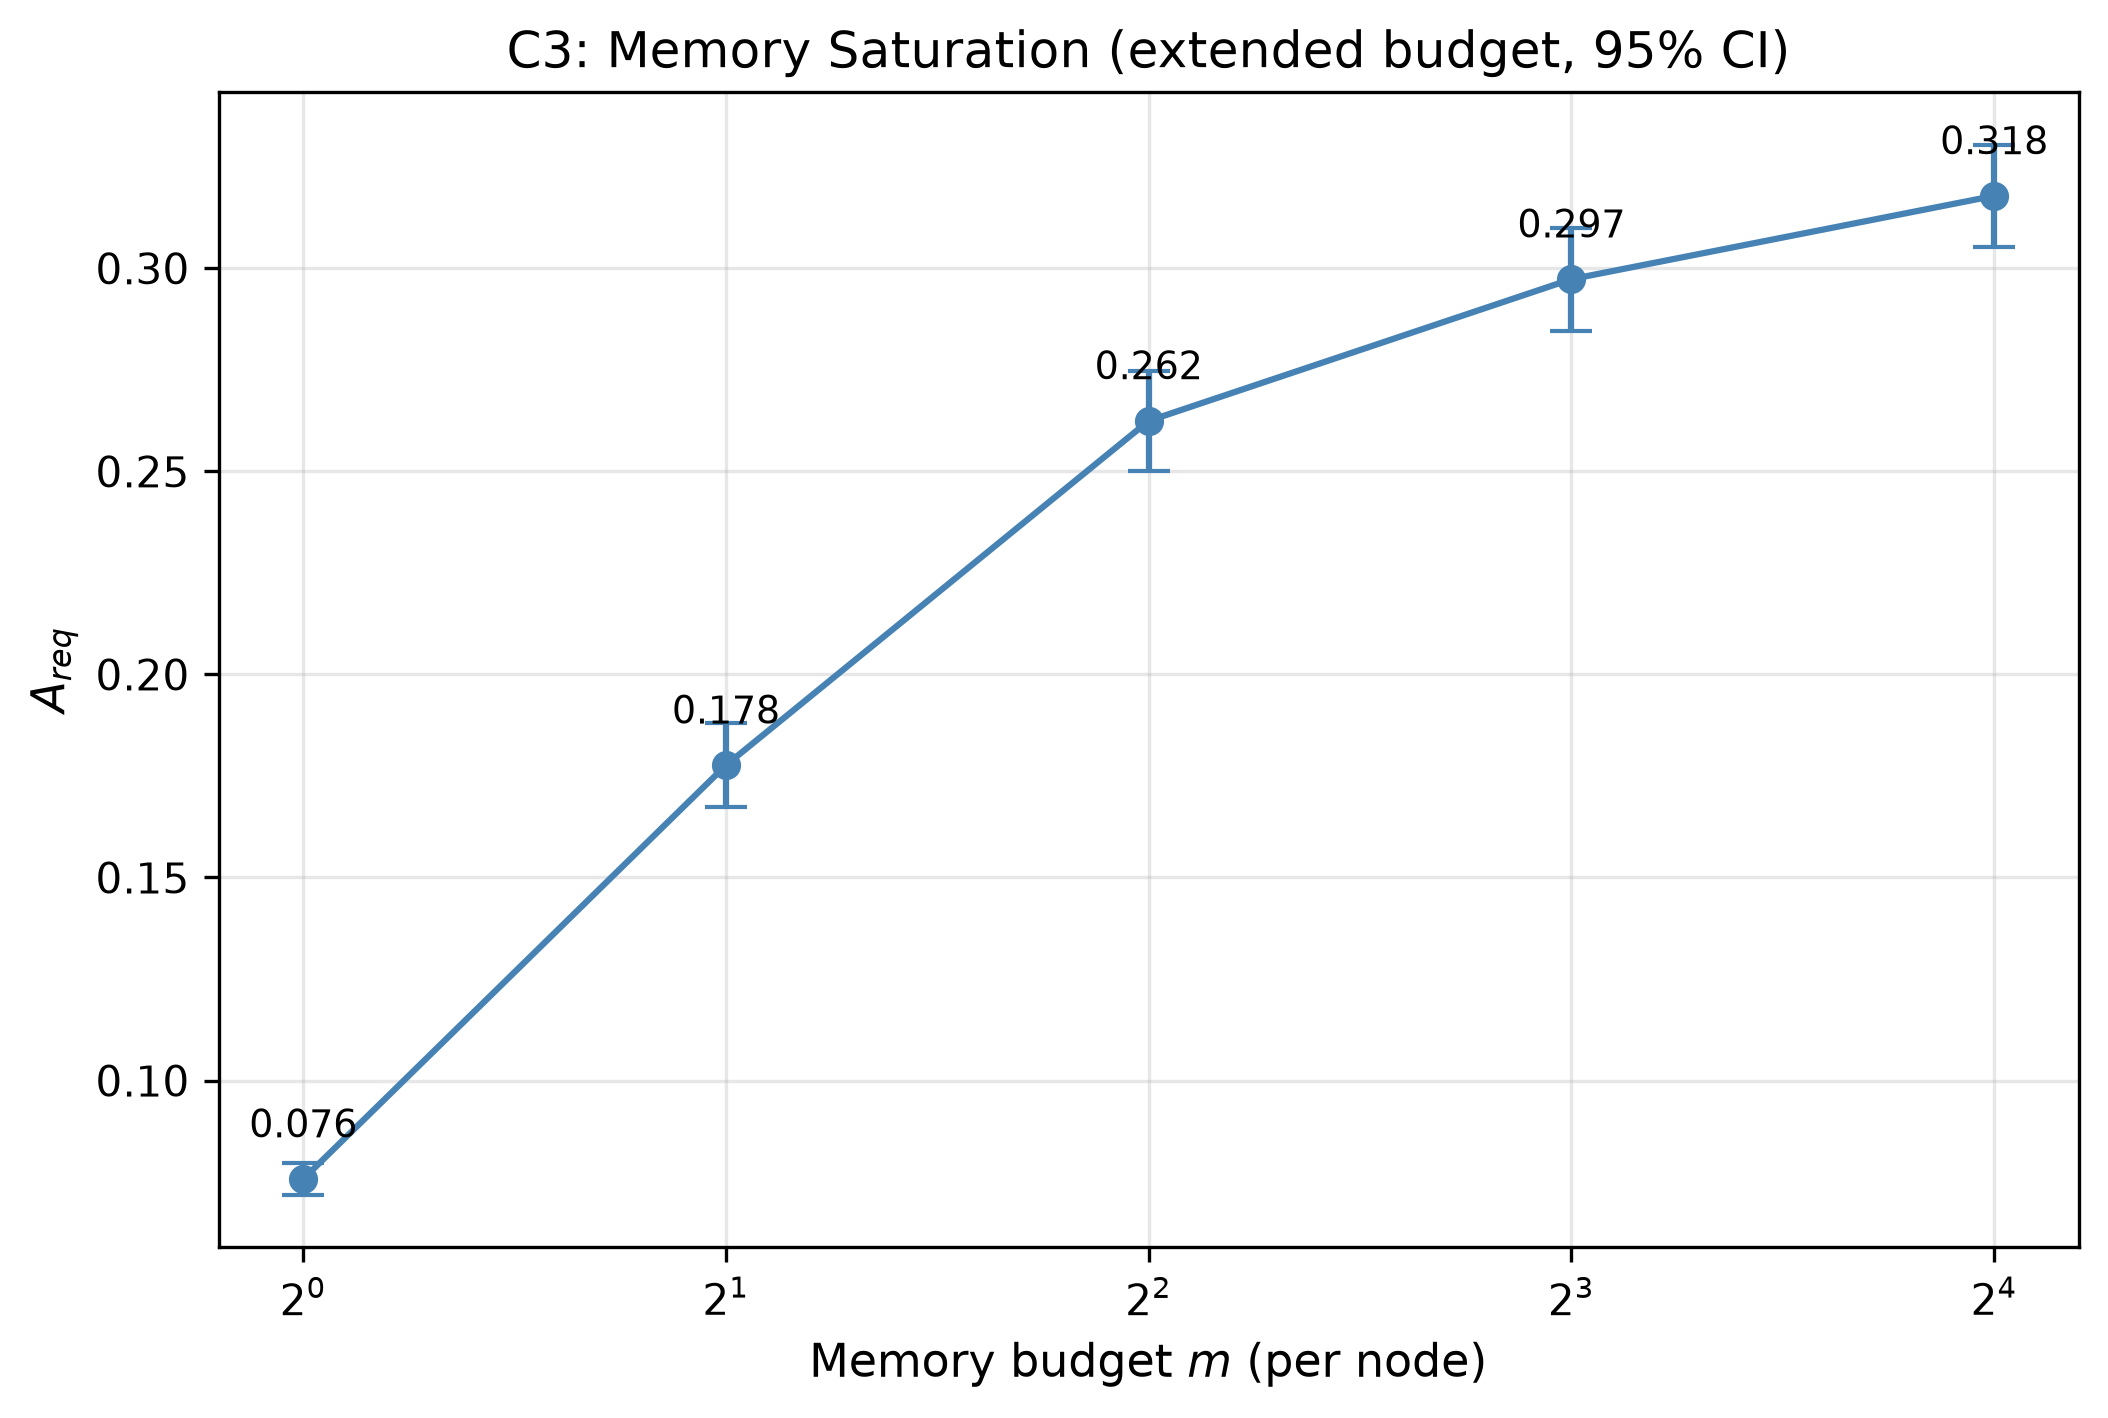
\includegraphics[width=0.95\columnwidth]{figures/fig_c3_extended.png}
\caption{C3 memory-budget response with extended budget ($m=1,2,4,8,16$, per node). Error bars show 95\% CI across 20 seeds. The curve flattens but does not reach a clear plateau within the tested range.}
\label{fig:c3_extended}
\end{figure}

\section{Memory-Budget Response and Memory-Budget Threshold}

\subsection{Budget-Response Curves}

Figure~\ref{fig:saturation} shows memory-budget response curves for four memory families across three topologies, using the per-node budget definition and an extended sweep $m \in \{1,2,4,8,16,32,64\}$.

\begin{figure*}[t]
\centering
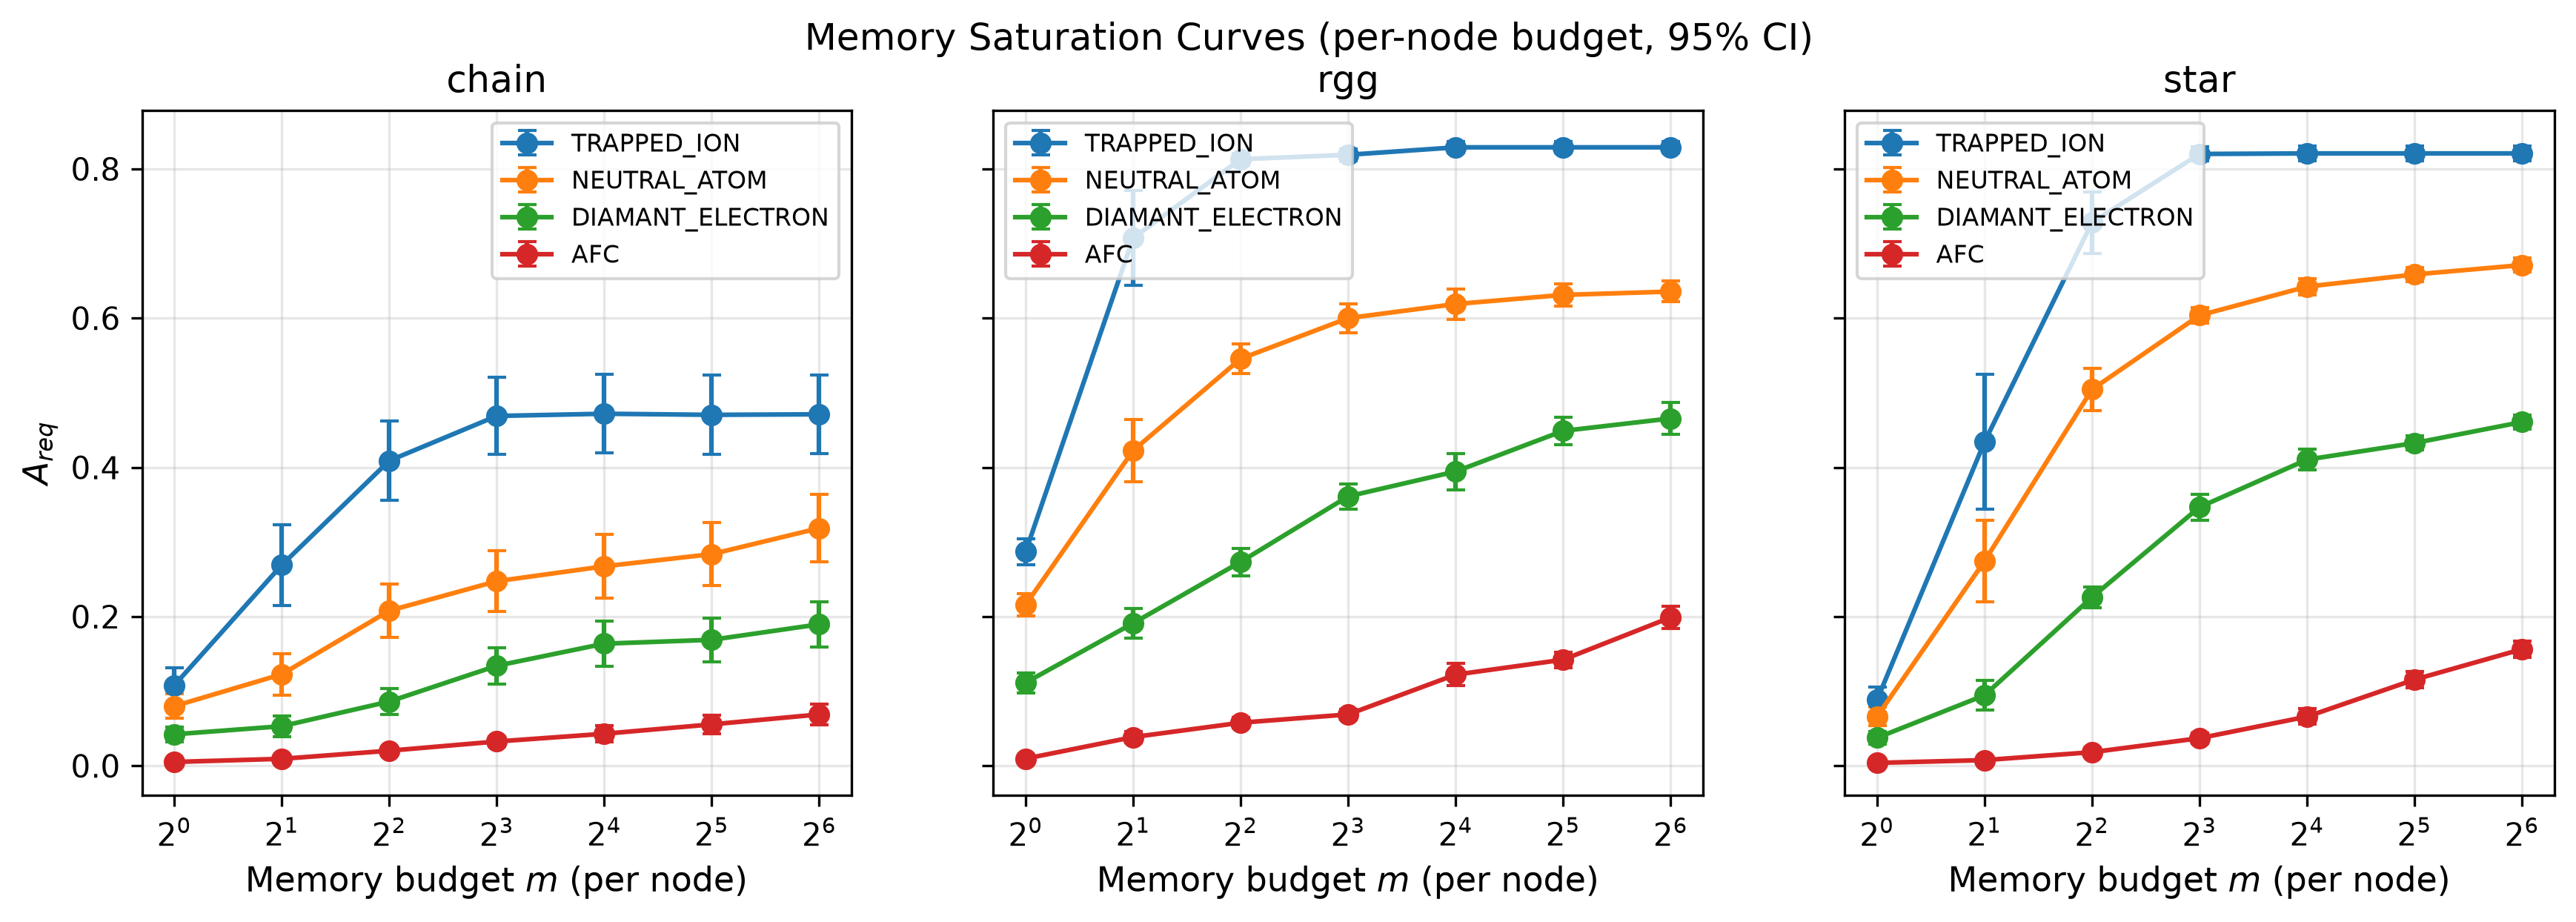
\includegraphics[width=0.98\textwidth]{figures/fig_saturation_v05.png}
\caption{Memory saturation curves with 95\% CI for four memory families across three topologies (per-node budget $m \in \{1,2,4,8,16,32,64\}$). Trapped-ion profiles approach a plateau within the tested range; AFC profiles are still increasing at $m=64$.}
\label{fig:saturation}
\end{figure*}

\subsection{Memory-Budget Threshold ($m_c$)}

We define the memory-budget threshold as the smallest per-node budget at which the primary performance metric $A_{\rm req}$ reaches a specified fraction of the best observed performance on the tested budget grid:
\begin{equation}
m_c(\alpha) = \min\left\{ m : A_{\rm req}(m) \geq \alpha \cdot A_{\max}^{\rm obs} \right\}
\end{equation}
with primary $\alpha = 0.95$. Here $A_{\max}^{\rm obs} = \max_m A_{\rm req}(m)$ is the maximum over the \emph{observed} budget grid $m \in \{1,2,4,8,16,32,64\}$, not an asymptotic limit. Because $A_{\max}^{\rm obs} > 0$ whenever any budget produces a nonzero signal, some budget on the grid always satisfies the criterion; the threshold is therefore always finite on the grid. We exclude regimes where $A_{\max}^{\rm obs} < 0.02$ (no meaningful signal), which removes 60 of the 900 profile--topology--traffic--size--seed combinations before the budget dimension. (The companion metric $A_{\rm qual}$ was used in the cross-implementation check because it showed stronger ordinal agreement across implementations, but the primary $m_c$ definition uses $A_{\rm req}$, consistent with the primary metric declared in Sec.~\ref{sec:model}.)

Three distinct concepts should not be conflated:
\begin{enumerate}[leftmargin=2em]
\item \textbf{Grid threshold:} The first budget on the discrete grid $\{1,2,4,8,16,32,64\}$ that reaches $\alpha \cdot A_{\max}^{\rm obs}$. This is what $m_c$ measures. A threshold at $m_c = 16$ does not imply that the minimum integer budget is exactly 16; the true minimum lies in $[8, 16]$ given the grid resolution.
\item \textbf{Practical plateau:} Whether the budget-response curve has flattened enough that further budget increases yield negligible improvement. This requires a separate plateau criterion (e.g., $|A(2m) - A(m)| < \delta$) and is not automatically established by $m_c$.
\item \textbf{Asymptotic threshold:} The threshold relative to an asymptotic performance level $A_\infty = \lim_{m \to \infty} A(m)$, if this limit can be identified. Our data do not identify a stable asymptote for all families; we therefore report grid thresholds, not asymptotic thresholds.
\end{enumerate}

Values reaching the upper boundary of the sweep ($m_c = 64$) indicate that the threshold was not reached at a lower budget on the grid. We label these as \textit{boundary cases} rather than ``right-censored,'' because the threshold relative to $A_{\max}^{\rm obs}$ is always defined on the grid; what is unknown is whether the curve would continue to rise beyond $m = 64$.

An audit across 4 families $\times$ 5 topologies $\times$ 3 traffic levels $\times$ 3 network sizes $\times$ 7 budgets $\times$ 5 seeds (6{,}300 nominal runs, of which 5{,}880 completed; 420 runs missing due to disconnected RGG graphs; 840 $m_c$ estimates at $\alpha=0.95$ after excluding 60 low-signal regimes; frozen file: \texttt{v05\_fixes/results/p1\_mc\_values.csv}) shows:

\begin{itemize}[leftmargin=2em]
\item $m_c = 1$: 0 regimes (0\%)
\item $m_c \leq 4$ (interior): 187 regimes (22.3\%)
\item $4 < m_c < 64$ (interior): 355 regimes (42.3\%)
\item Boundary case ($m_c = 64$): 298 regimes (35.5\%)
\end{itemize}

Table~\ref{tab:mc_family} shows the per-family $m_c$ distribution, and Figure~\ref{fig:mc} visualizes the overall distribution.

\begin{table}[htbp]
\centering
\caption{Per-family $m_c$ at $\alpha=0.95$ (per-node budget). ``Boundary'' indicates $m_c = 64$.}
\label{tab:mc_family}
\begin{tabular}{lrrrr}
\toprule
Family & Median $m_c$ & Range & Boundary & $n$ \\
\midrule
Trapped Ion & 4 & [2, 16] & 0/210 & 210 \\
Neutral Atom & 16 & [4, 64] & 52/210 & 210 \\
Diamond (Electron) & 32 & [8, 64] & 102/210 & 210 \\
AFC & $\geq 64$ & [2, $\geq 64$] & 144/210 & 210 \\
\bottomrule
\end{tabular}
\end{table}

The threshold location varies strongly by memory profile: the Trapped Ion profile reaches the 95\%-of-observed-maximum threshold at a median $m_c=4$, while AFC reaches the boundary ($m_c = 64$) in 69\% of its regimes. Because 35.5\% of observations are boundary cases, we do not report a single mean or standard deviation for $m_c$. The data support a regime-dependent threshold, not a universal constant. These $m_c$ estimates are model-specific quantitative results of the WestQuant simulation; a coarser cross-implementation sweep reproduced the qualitative regime-dependence of the memory threshold but showed sensitivity of threshold location to implementation details. Direct quantitative cross-validation of the full $m=\{1,2,4,8,16,32,64\}$ threshold analysis remains future work.

\textbf{$\alpha$ stability:} The median $m_c$ increases from 16 ($\alpha=0.90$) to 32 ($\alpha=0.95$ and $0.99$), indicating that the threshold is moderately sensitive to the saturation criterion.

\begin{figure*}[t]
\centering
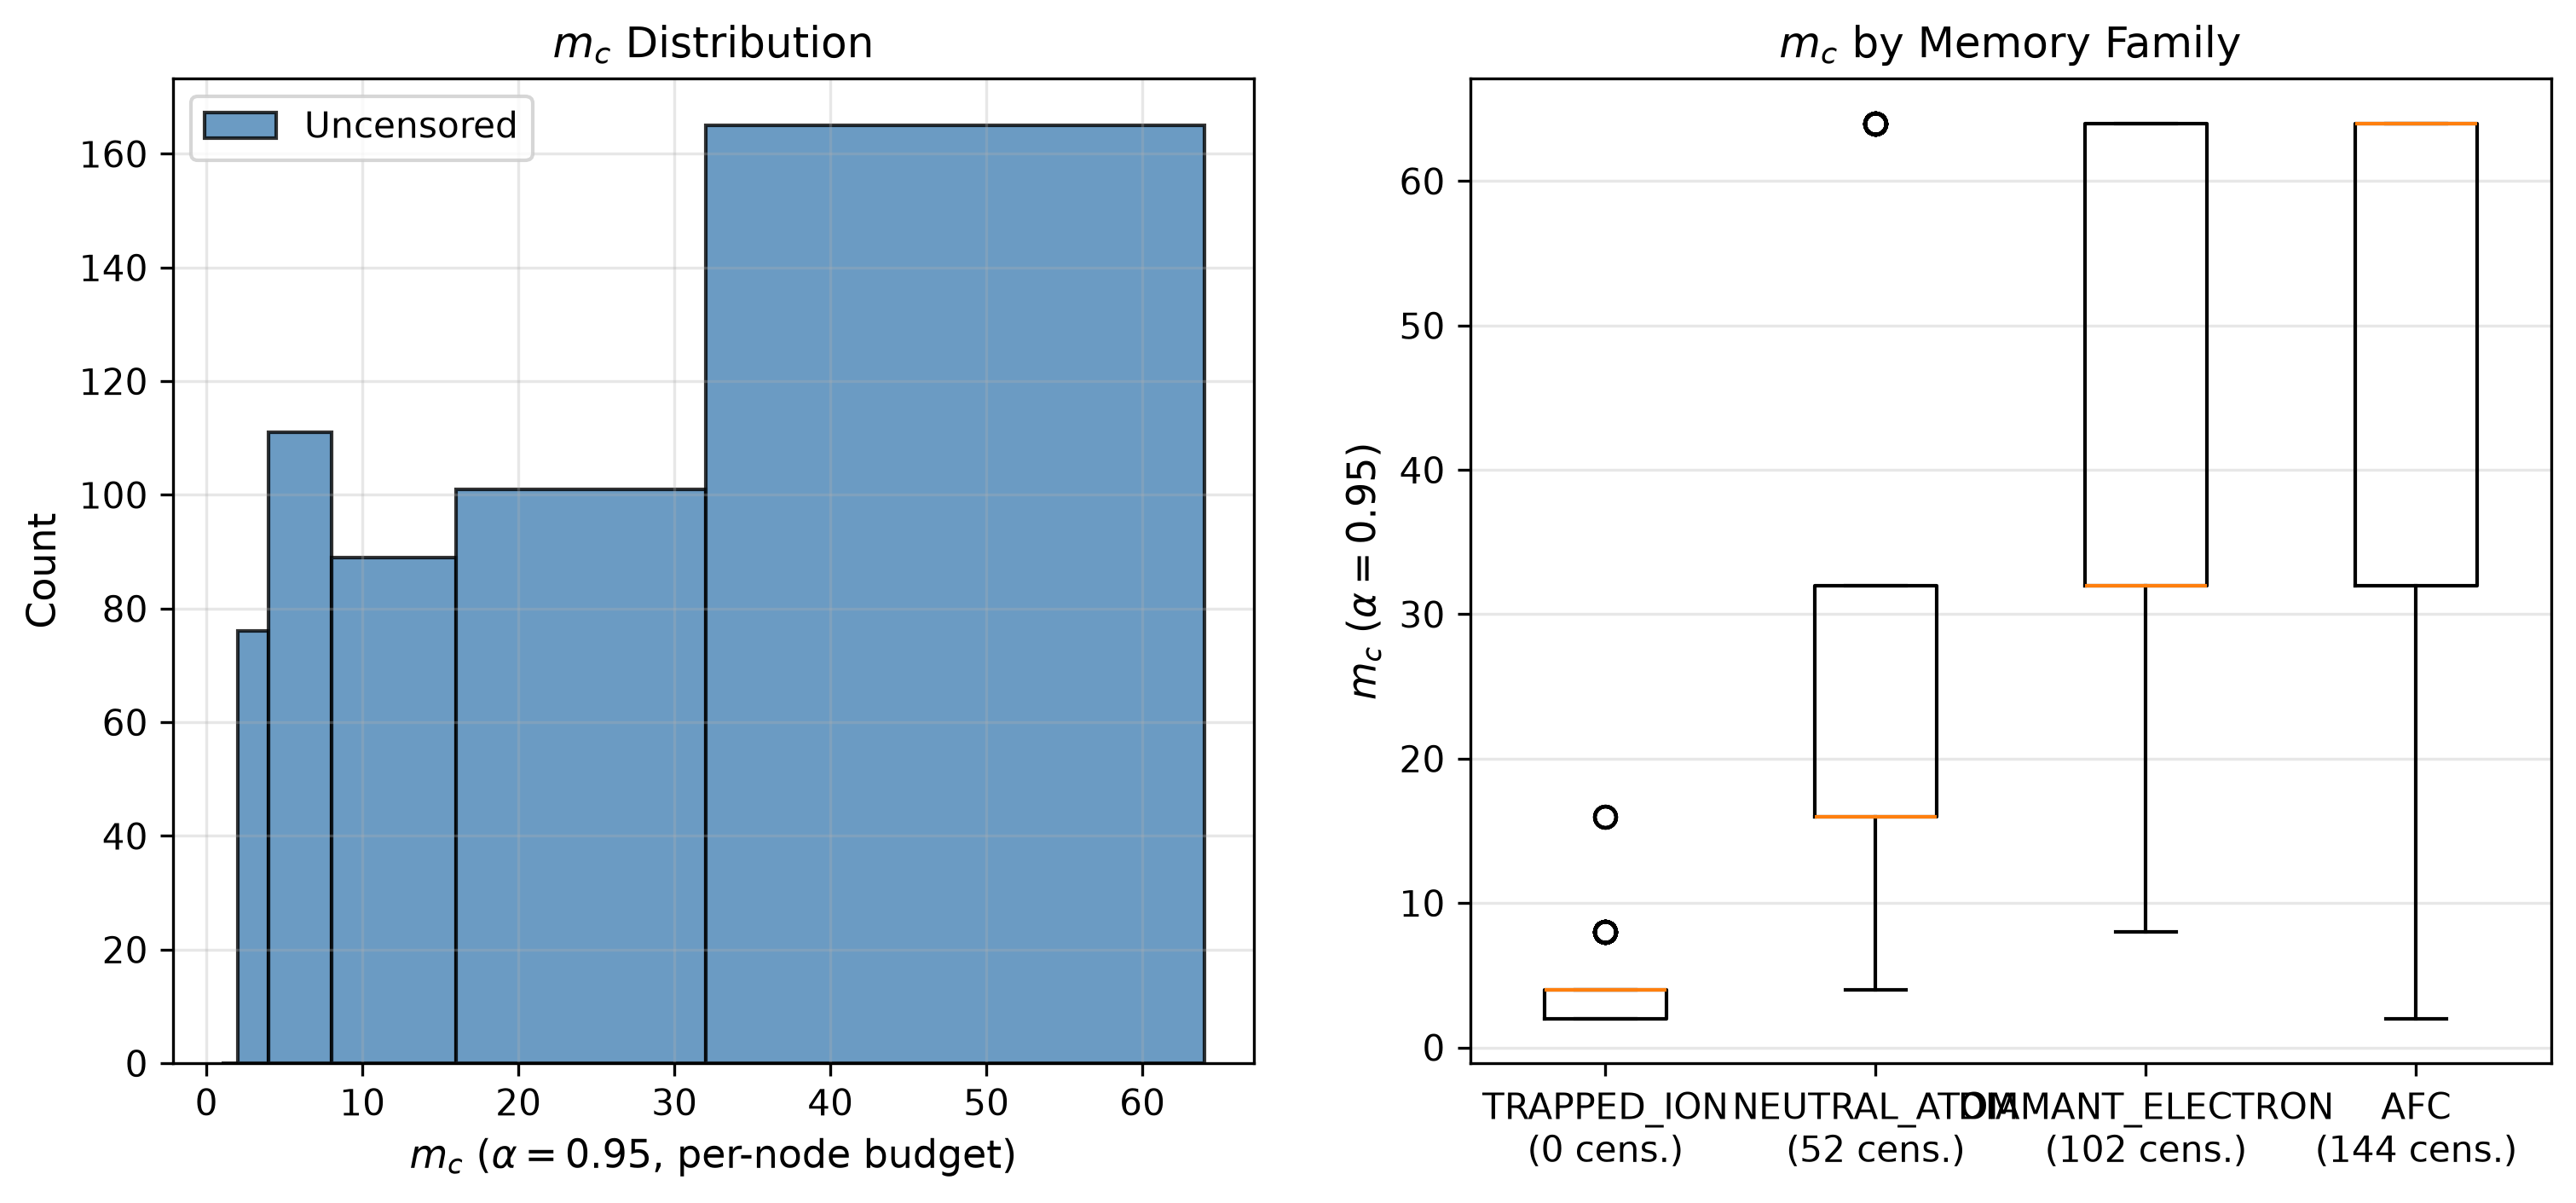
\includegraphics[width=0.98\textwidth]{figures/fig_mc_distribution_v05.png}
\caption{(Left) $m_c$ distribution at $\alpha=0.95$ (per-node budget). Boundary cases ($m_c = 64$) are shown in red. (Right) $m_c$ by memory family; boundary counts are annotated.}
\label{fig:mc}
\end{figure*}

\section{Failure of Universal Scalar Scaling}

We test four dimensionless scaling hypotheses. The first three are motivated by dimensional analysis of the load--capacity ratio and its topology corrections; the fourth incorporates memory physics:

\begin{align}
\Pi &= \frac{\lambda \, t_{\rm attempt}}{m \, p_{\rm gen}} \\
\Pi^* &= \Pi \cdot \sqrt{\bar{h}} \\
\Pi_B &= \max_v \rho_v, \quad \rho_v = \frac{\Lambda_v}{m_v \cdot \mu}, \quad \mu = \frac{p_{\rm gen}}{t_{\rm attempt}} \\
\Pi_{\rm phys} &= \frac{\Pi}{\eta_r \cdot \exp(-t_{\rm storage}/T_2)}
\end{align}

where $\bar{h}$ is the mean shortest-path length, $\Lambda_v$ is the traffic-weighted betweenness of node $v$, $m_v$ is the memory at node $v$, and $t_{\rm storage}$ is the mean storage time. $\Pi_B$ is the maximum node utilization (bottleneck-flow parameter). $\Pi_{\rm phys}$ incorporates retrieval efficiency $\eta_r$ and coherence decay.

\textbf{Quantitative test:} We compute the coefficient of determination $R^2$ for $A_{\rm req}$ as a function of each scalar (log-transformed). All four candidates are evaluated in the pooled data; $\Pi$, $\Pi_B$, and $\Pi_{\rm phys}$ are also evaluated separately within each memory profile (Table~\ref{tab:r2}):

\begin{table}[htbp]
\centering
\caption{$R^2$ of $A_{\rm req}$ versus the three candidates evaluated per profile. $\Pi^*$ was evaluated in the pooled global collapse test ($R^2=0.042$) but was not separately refit per profile in the frozen closure analysis.}
\label{tab:r2}
\begin{tabular}{lrrr}
\toprule
Profile & $R^2(\Pi)$ & $R^2(\Pi_B)$ & $R^2(\Pi_{\rm phys})$ \\
\midrule
Trapped Ion & 0.153 & 0.255 & 0.245 \\
Neutral Atom & 0.081 & 0.176 & 0.166 \\
Diamond (Electron) & 0.040 & 0.123 & 0.112 \\
Diamond (Nuclear) & 0.024 & 0.103 & 0.085 \\
AFC & 0.017 & 0.084 & 0.067 \\
Superconducting & 0.007 & 0.042 & 0.000 \\
\midrule
Pooled $R^2$ & 0.025 & 0.052 & 0.177 \\
\bottomrule
\end{tabular}
\end{table}

Among the three candidates evaluated per profile, no scalar achieves $R^2 > 0.26$; all four candidates have pooled $R^2<0.18$. For $\Pi$ alone, 85--99\% of within-profile response variance remains unexplained, and Figure~\ref{fig:scalar} shows that the residual structure is visibly organized into topology-specific bands. Table~\ref{tab:topo_residual} quantifies the unexplained fraction per profile.

\begin{table}[htbp]
\centering
\caption{Fraction of within-profile response variance unexplained by the log-$\Pi$ regression, computed as $1-R^2(\Pi)$. This quantity is residual variance, not a direct variance-component estimate for topology.}
\label{tab:topo_residual}
\begin{tabular}{lr}
\toprule
Profile & Unexplained fraction $1-R^2(\Pi)$ \\
\midrule
Trapped Ion & 0.847 \\
Neutral Atom & 0.919 \\
Diamond (Electron) & 0.960 \\
Diamond (Nuclear) & 0.976 \\
AFC & 0.983 \\
Superconducting & 0.994 \\
\bottomrule
\end{tabular}
\end{table}

Figure~\ref{fig:scalar} shows the scalar collapse test, and Figure~\ref{fig:r2} compares the $R^2$ values across families.

\begin{figure*}[t]
\centering
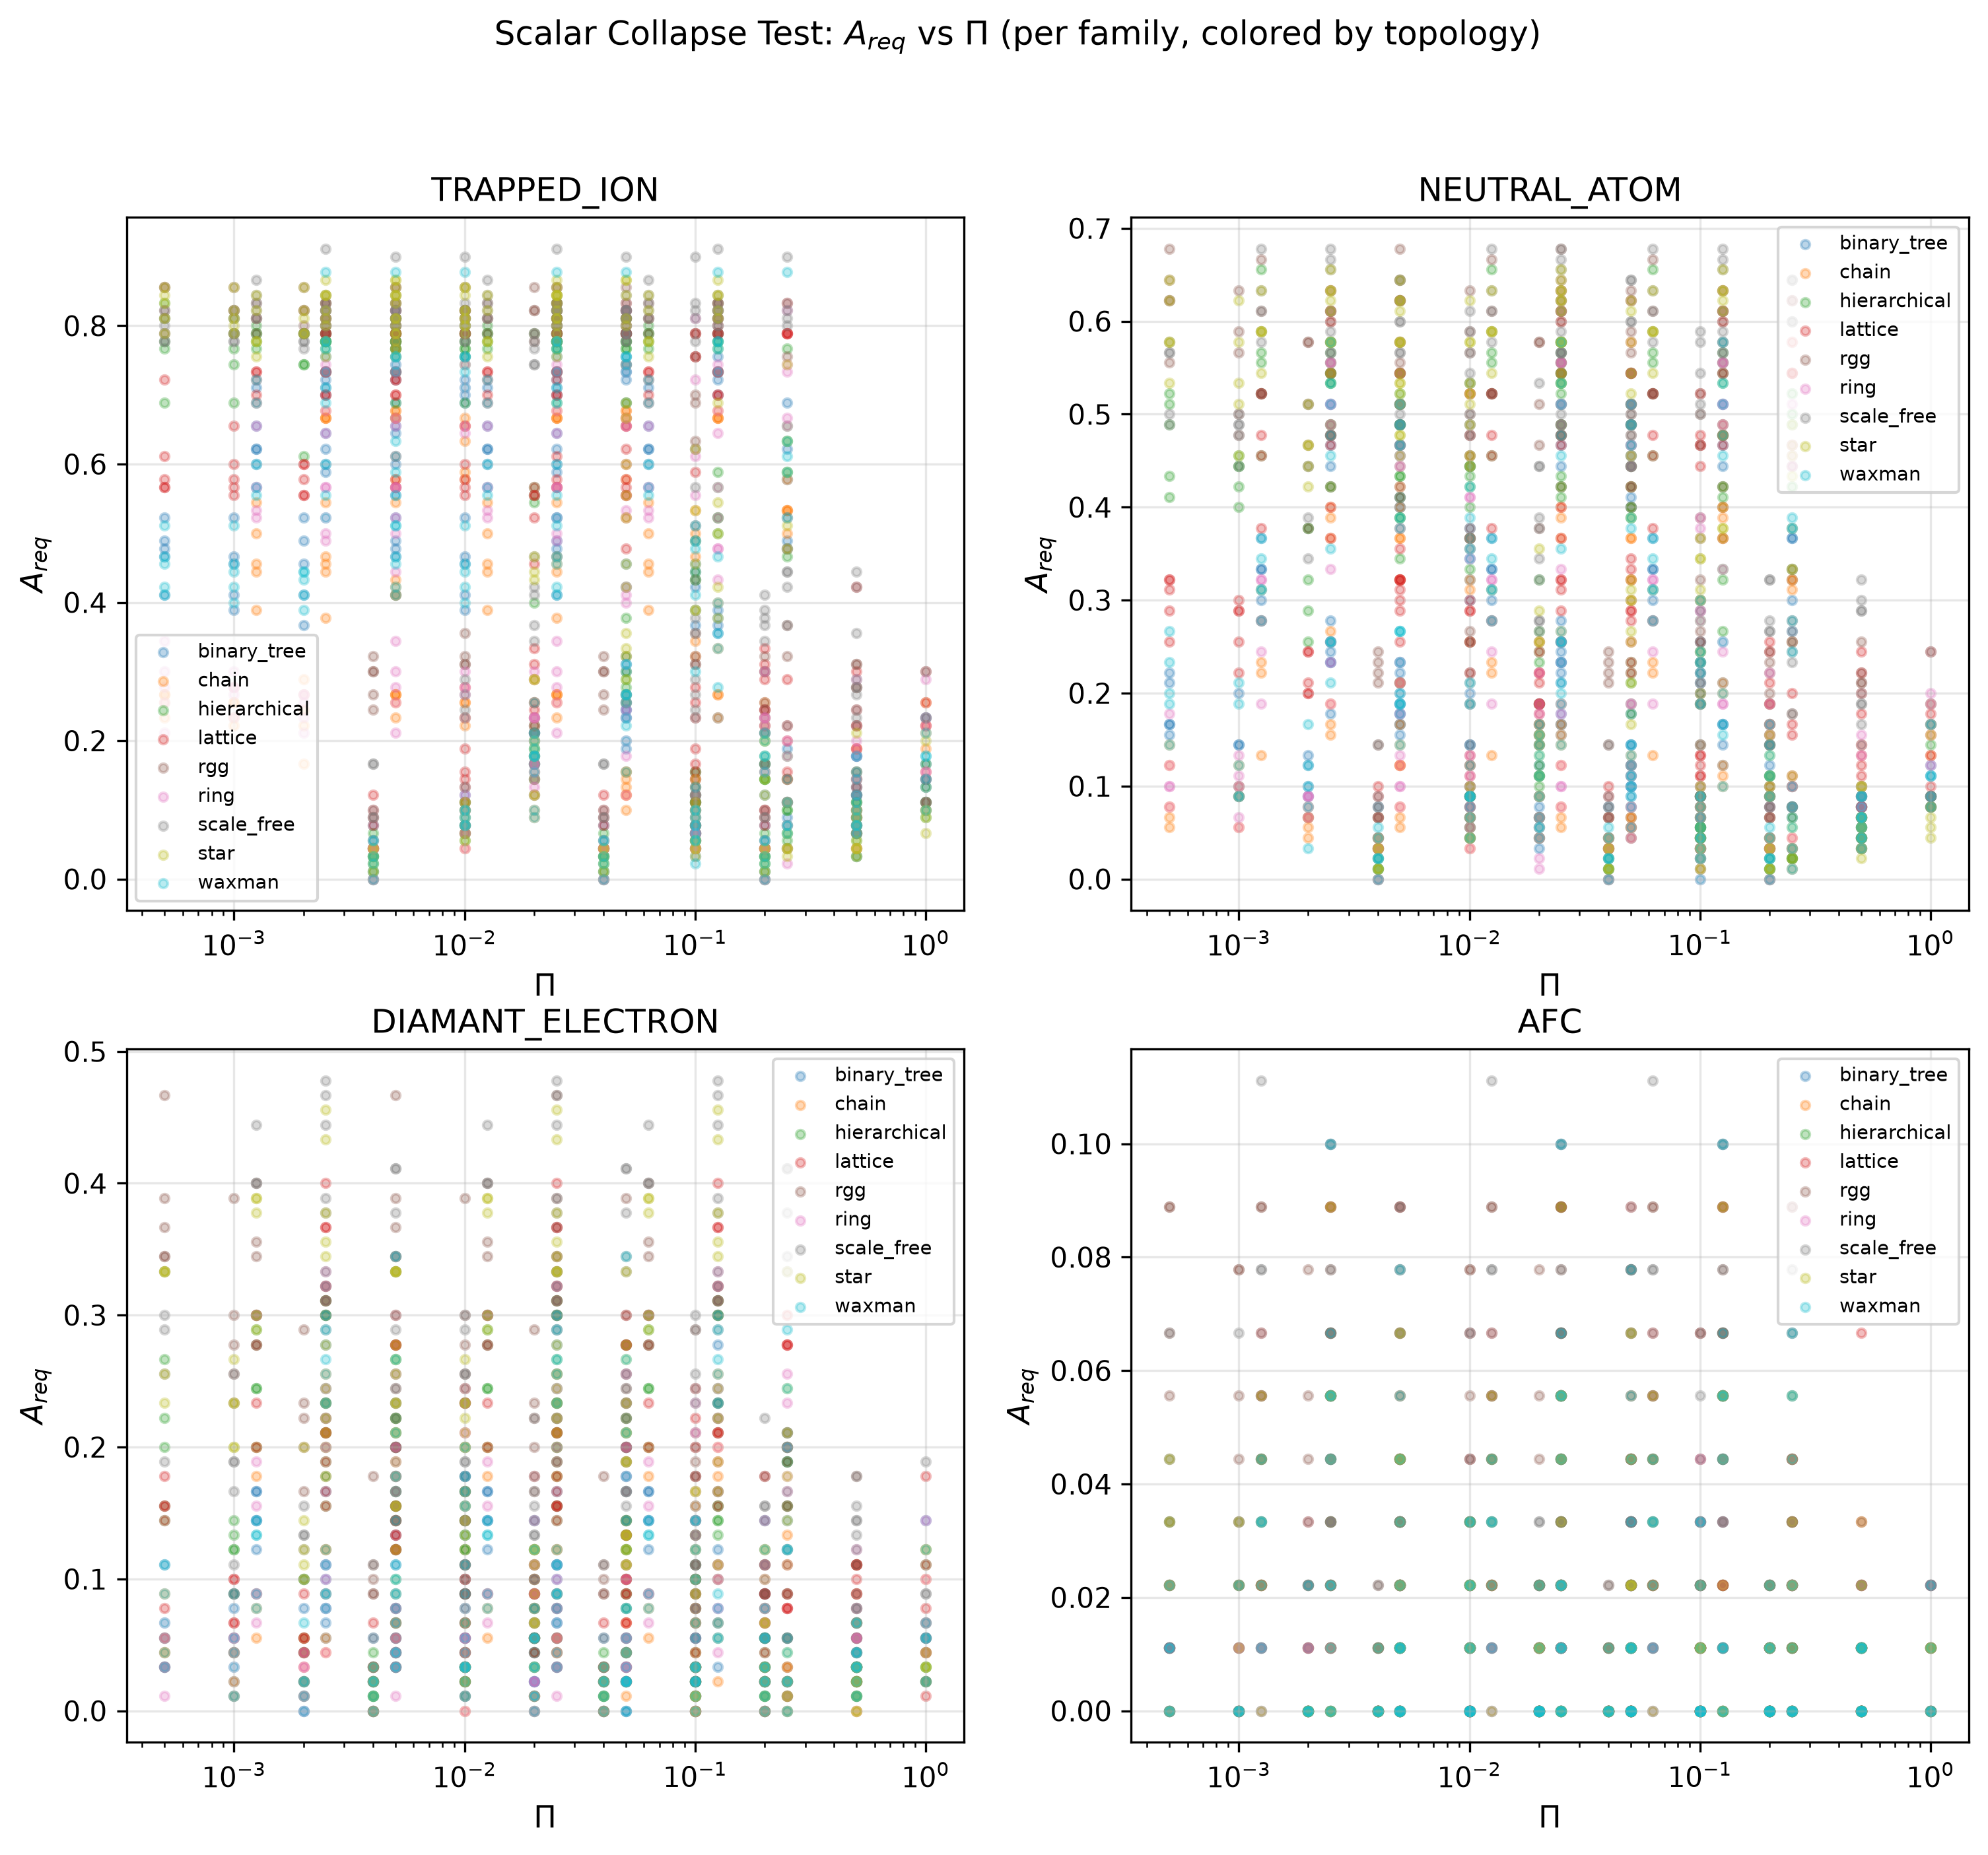
\includegraphics[width=0.85\textwidth]{figures/fig_scalar_collapse_v05.png}
\caption{Scalar collapse test: $A_{\rm req}$ vs $\Pi$ for four memory families, colored by topology. Topology-specific bands persist within each family, confirming that $\Pi$ does not capture topology-dependent variation even when hardware is held fixed.}
\label{fig:scalar}
\end{figure*}

\begin{figure}[t]
\centering
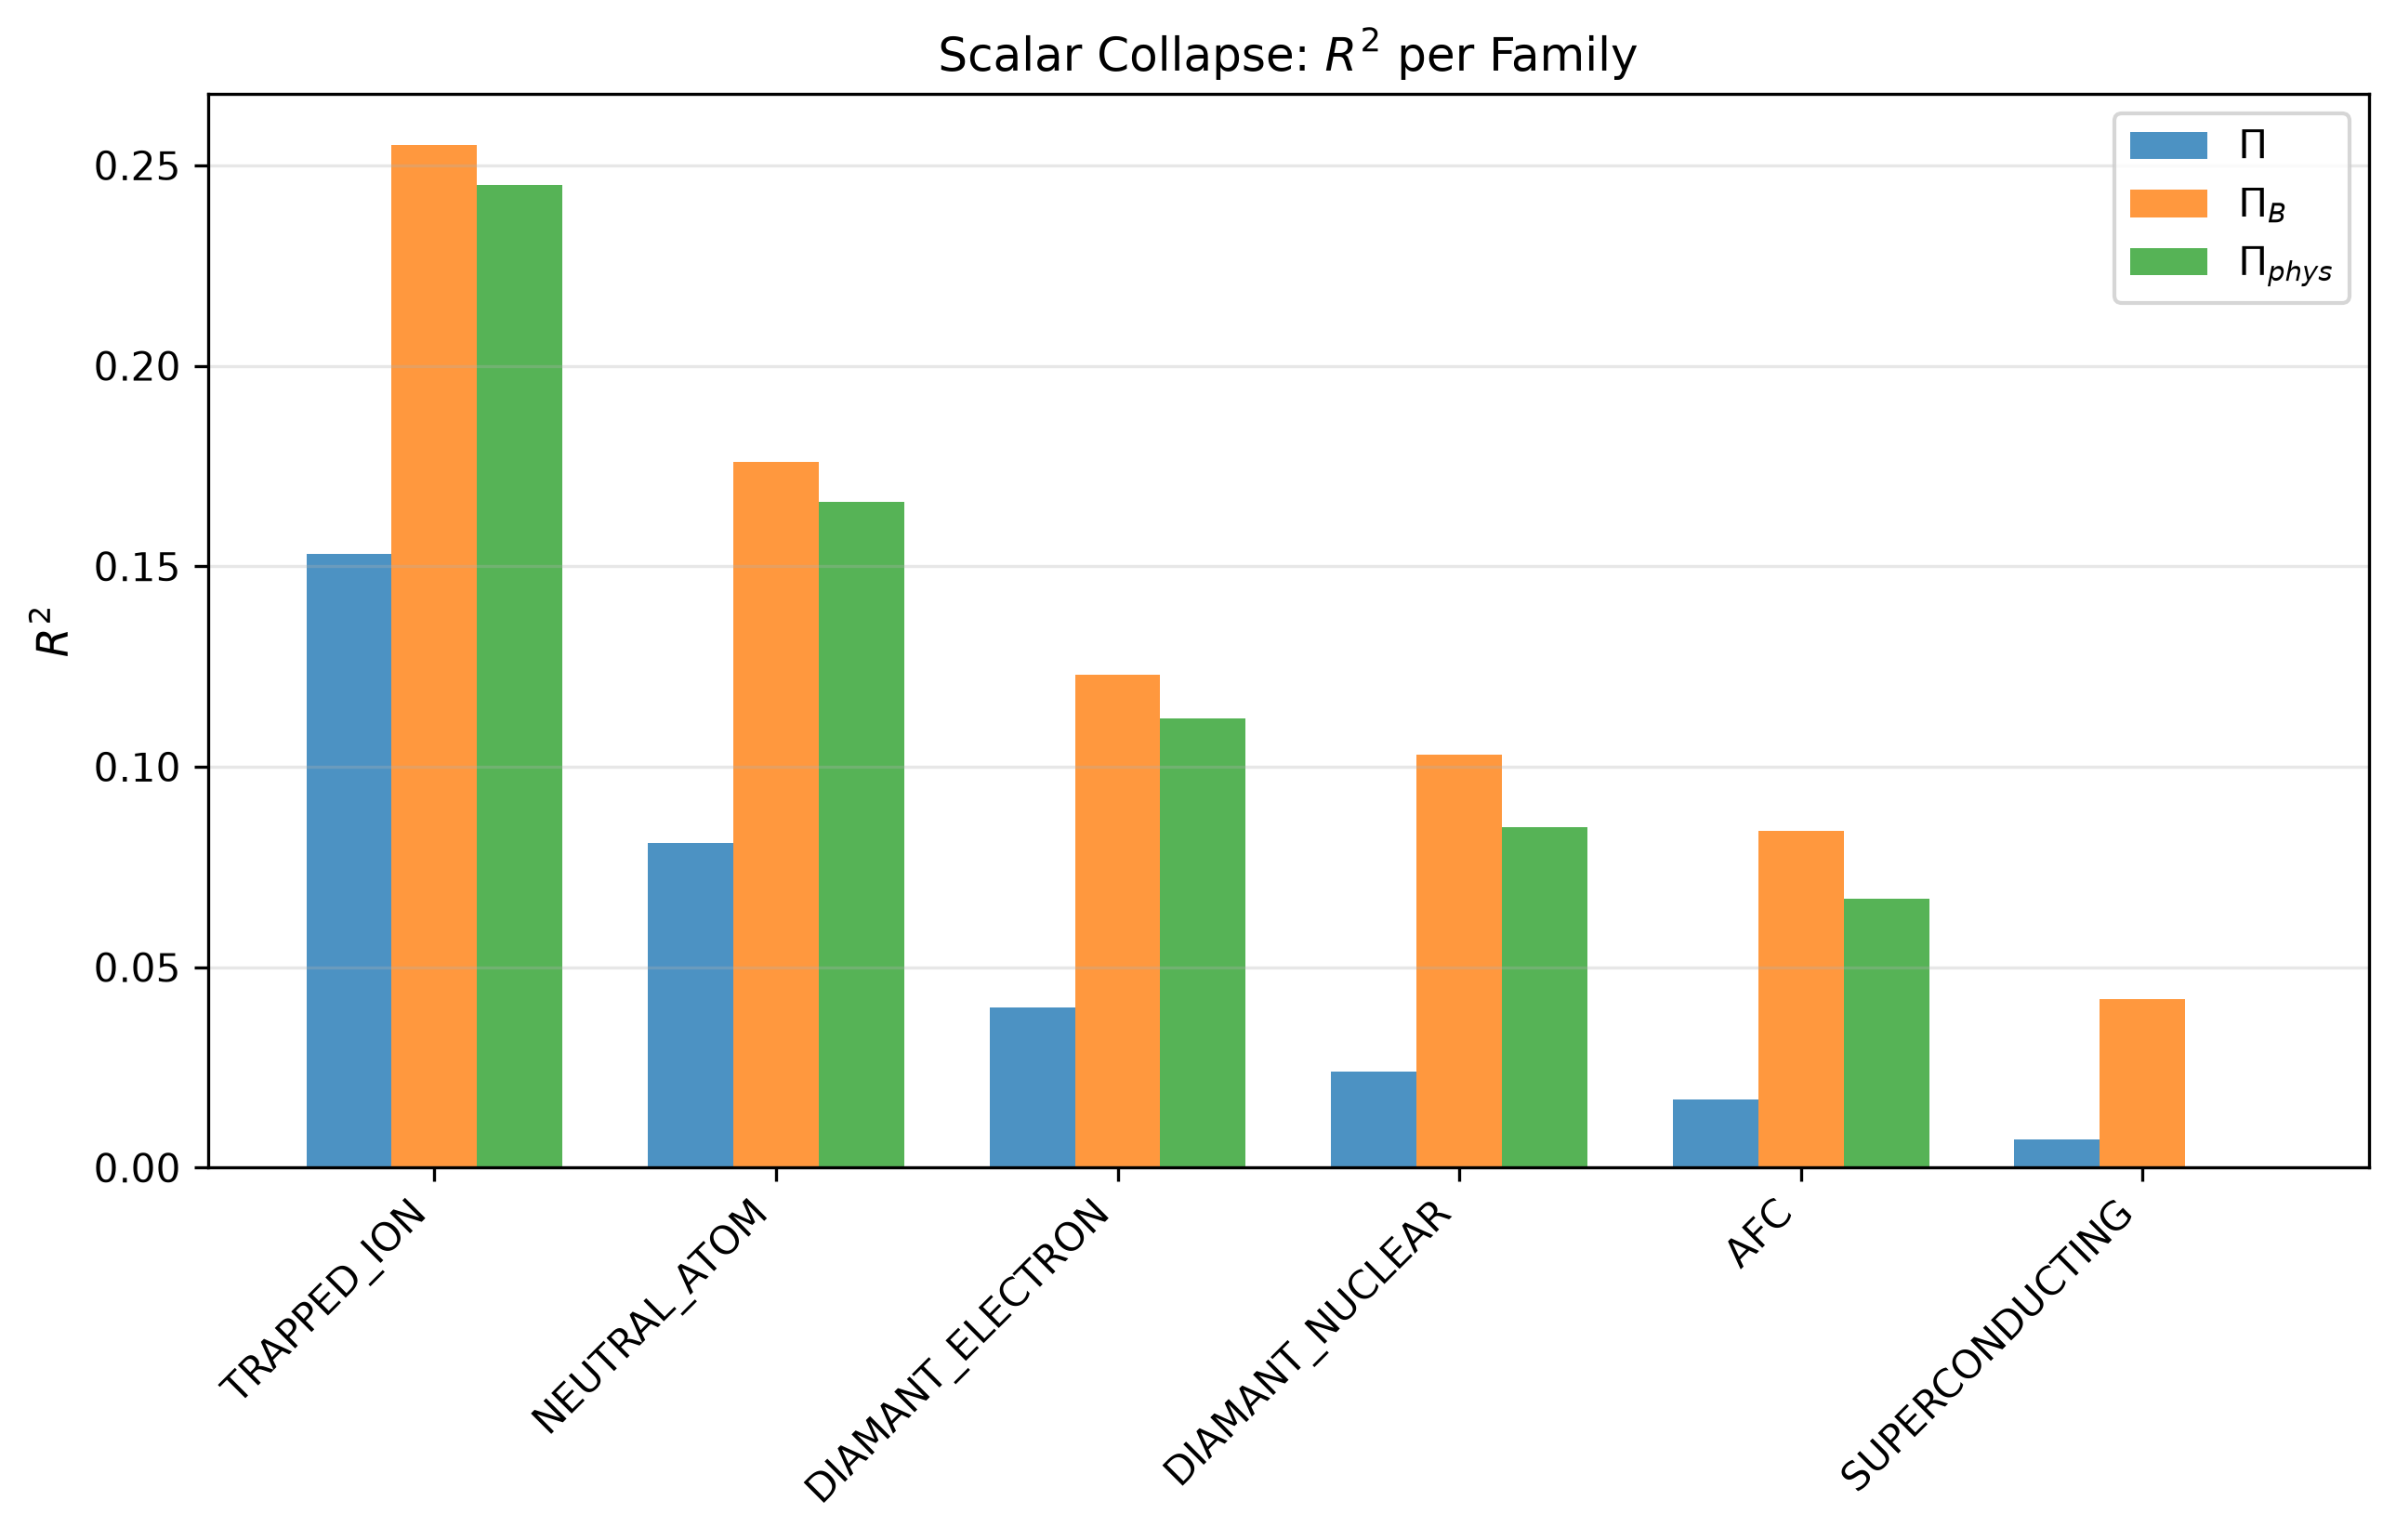
\includegraphics[width=0.95\columnwidth]{figures/fig_r2_comparison.png}
\caption{$R^2$ per family for $\Pi$, $\Pi_B$, and $\Pi_{\rm phys}$. No scalar exceeds $R^2 = 0.26$ in any family.}
\label{fig:r2}
\end{figure}

\textbf{Claim:} In the WestQuant dataset, none of the four tested scalar reductions achieves a topology- and hardware-independent collapse. We do not claim that no universal scaling law can ever exist---only that these specific candidates are insufficient. The physics-aware candidate $\Pi_{\rm phys}$ achieves the highest overall $R^2$ (0.177) but still leaves more than 82\% of variance unexplained. The scalar-collapse result has not yet been independently cross-implemented.

\textbf{Nonlinear collapse test:} Because the linear $R^2$ test may miss a nonlinear monotonic relationship, we additionally compute (i)~Spearman rank correlation $\rho_s$ between each scalar and $A_{\rm req}$, and (ii)~$R^2$ of a quadratic log-transformed fit $A_{\rm req} = a(\log \Pi)^2 + b\log\Pi + c$. Table~\ref{tab:nonlinear} reports the pooled results. For $\Pi$, $\Pi^*$, and $\Pi_B$, the quadratic $R^2$ remains below 0.06 and $|\rho_s| < 0.22$, confirming that both linear and nonlinear monotonic fits fail. For $\Pi_{\rm phys}$, the quadratic fit improves to $R^2 = 0.379$ (pooled) with $\rho_s = -0.721$, but per-family quadratic $R^2$ remains below 0.28 (Trapped Ion: 0.274; AFC: 0.069), indicating that the pooled improvement is driven by inter-family separation rather than within-family collapse. We therefore conclude that the failure of universal scalar scaling is robust to nonlinear monotonic transformations for $\Pi$, $\Pi^*$, and $\Pi_B$, and that $\Pi_{\rm phys}$ shows partial nonlinear improvement but does not achieve a topology-independent within-profile collapse.

\begin{table}[htbp]
\centering
\caption{Nonlinear scalar-collapse test (pooled). $R^2_{\rm lin}$: linear log-transformed. $R^2_{\rm quad}$: quadratic log-transformed. $\rho_s$: Spearman rank correlation.}
\label{tab:nonlinear}
\begin{tabular}{lrrr}
\toprule
Scalar & $R^2_{\rm lin}$ & $R^2_{\rm quad}$ & $\rho_s$ \\
\midrule
$\Pi$ & 0.025 & 0.029 & $-0.118$ \\
$\Pi^*$ & 0.042 & 0.045 & $-0.169$ \\
$\Pi_B$ & 0.052 & 0.058 & $-0.214$ \\
$\Pi_{\rm phys}$ & 0.177 & 0.379 & $-0.721$ \\
\bottomrule
\end{tabular}
\end{table}

\FloatBarrier

\section{Retrieval-Window Descriptor and Limits of Analytical Sizing}
\label{sec:chi_law}

The four scalar candidates above fail to predict $m_c$ without circularity. We now examine the retrieval-window parameter $\chi_r = \tau_r\, p_{\rm gen} / t_{\rm attempt}$ (defined in Eq.~\ref{eq:chi}), where $\tau_r$ is the retrieval decay time, as a physical descriptor of the operating regime. We present an independent-channel reference calculation, discuss its physical interpretation, and identify the limits of analytical sizing. No predictive accuracy or invariance rate is asserted for the corrected $\chi_r$ in this revision; the calculation below is an illustrative reference, not a validated predictor.

\subsection{Independent-Channel Reference Calculation}

For a single link, the number of link attempts within one retrieval lifetime is
\begin{equation}
K = \left\lfloor \frac{\tau_r}{t_{\rm attempt}} \right\rfloor \,,
\end{equation}
and the probability of at least one successful generation within the retrieval lifetime is
\begin{equation}
p_w = 1 - (1 - p_{\rm gen})^{K} \,.
\end{equation}
The memory budget needed to achieve target availability $\alpha$ on a single link is
\begin{equation}
m_{\rm single} \approx \frac{\ln(1-\alpha)}{\ln(1 - p_w)} \,.
\end{equation}
Table~\ref{tab:chi_single} compares the single-link reference calculation to the observed median $m_c$ across the four primary profiles.

\begin{table}[htbp]
\centering
\caption{Single-link reference calculation vs.\ observed median $m_c$ at $\alpha=0.95$ (per-node budget). Observations are 2--3$\times$ higher than the single-link reference, consistent with multi-hop paths requiring simultaneous link success. The reference is illustrative, not a validated predictor.}
\label{tab:chi_single}
\begin{tabular}{lrrrr}
\toprule
Profile & $\chi_r$ & $p_w$ & Reference $m$ & Observed median \\
\midrule
Trapped Ion & 50 & $\approx 1$ & 1 & 4 \\
Neutral Atom & 0.5 & 0.39 & 6 & 16 \\
Diamond (Electron) & 0.22 & 0.20 & 14 & 32 \\
AFC & 0.025 & 0.025 & 120 & 64 \\
\bottomrule
\end{tabular}
\end{table}

The single-link reference underestimates the observed $m_c$ by a factor of 2--3. This is expected: in multi-hop networks, all $h$ links along a path must succeed, so the effective path-success probability is $p_{\rm path} = p_w^{\,h}$, which is much smaller than $p_w$ and therefore requires more memory budget.

\subsection{Multi-Hop Reference and AFC Illustrative Example}

For a path of $h$ hops, the memory threshold becomes
\begin{equation}
m_{\rm multi}(h) \approx \frac{\ln(1-\alpha)}{\ln(1 - p_w^{\,h})} \,.
\end{equation}
As an illustrative reference, consider the AFC profile ($\tau_r = 0.01$~s, $p_{\rm gen} = 0.005$, $t_{\rm attempt} = 10^{-3}$~s) on a 2-hop path at $\alpha = 0.95$:
\begin{itemize}[leftmargin=2em]
\item $K = \lfloor 0.01 / 0.001 \rfloor = 10$ attempts per retrieval lifetime
\item $p_w = 1 - (1 - 0.005)^{10} \approx 0.0489$
\item $p_{\rm path} = p_w^{2} \approx 0.00239$
\item $m_{\rm multi}(2) = \ln(0.05) / \ln(1 - 0.00239) \approx 1252$ channels
\end{itemize}
This $\sim$1252-channel figure is an illustrative reference for the coincidence-limited regime, not a validated prediction of the observed $m_c$. The observed AFC median $m_c \geq 64$ (Table~\ref{tab:mc_family}) is lower than this reference, which does not account for topology-specific path lengths, traffic, or contention effects captured in the simulation.

\subsection{Physical Interpretation}

The $\chi_r$ values cleanly separate the four primary profiles into two regimes (Table~\ref{tab:chi_regimes}):
\begin{itemize}[leftmargin=2em]
\item \textbf{Queue-limited} ($\chi_r \gg 1$, Trapped Ion $\chi_r = 50$): Many link successes occur within the memory lifetime, so the bottleneck is queueing and contention, not coincidence. Memory demand is governed by Little's law.
\item \textbf{Coincidence-limited} ($\chi_r \ll 1$, AFC $\chi_r = 0.025$, Diamond Electron $\chi_r = 0.22$): Link success within the memory lifetime is rare. Memory demand is governed by the coincidence probability $p_w$, and $m_c$ is large.
\item \textbf{Transitional} ($\chi_r \sim 1$, Neutral Atom $\chi_r = 0.5$): Both mechanisms contribute.
\end{itemize}

This regime separation is consistent with the per-family $m_c$ distribution (Table~\ref{tab:mc_family}): Trapped Ion (queue-limited) has median $m_c = 4$, while AFC (coincidence-limited) has median $m_c \geq 64$. The retrieval-window descriptor thus provides a physical interpretation for the regime-dependent threshold that the four scalar candidates could not capture without circularity.

\textbf{No predictive accuracy or invariance rate is asserted.} The independent-channel approximation does not account for topology, traffic, contention, or interface effects. No invariance test, factorial variance attribution, or benchmark comparison is reported for the corrected $\chi_r$ in this revision. The descriptor is offered as a physical timescale interpretation, not as a network memory-sizing law.

\FloatBarrier

\section{Heterogeneous Memory Placement}
\label{sec:heterogeneity}

We resolve an apparent contradiction in earlier exploratory results with a controlled experiment over 6 topologies, 2 network sizes, 3 traffic levels, 3 coupling rules, and 5 seeds. Four mixed-placement strategies are evaluated at both high-quality fractions, while the two homogeneous controls (all-high and all-low) are evaluated once per graph/traffic/coupling condition. This gives 5{,}400 nominal runs. Ninety runs (1.7\%) are skipped due to disconnected RGG graphs at $N=20$, leaving 5{,}310 actual runs.

\textbf{Definitions:} \textit{Hub} nodes are the top-$k$ nodes by degree centrality. \textit{Bottleneck} nodes are the top-$k$ nodes by betweenness centrality. \textit{Peripheral} nodes are the bottom-$k$ nodes by degree centrality. In a star topology, the hub and bottleneck nodes coincide.

\textbf{Result:} Hubs (mean $A=0.0815$) and bottlenecks (mean $A=0.0766$) outperform peripheral placement (mean $A=0.0323$). The strategy ranking is robust across coupling rules (Kendall $\tau = 1.0$ for all pairs of \{min, sqrt, product\}).

\textbf{Paired comparison (hub vs bottleneck):} Across 1{,}062 matched pairs, the median paired difference is 0 (558 ties, 322 hub wins, 182 bottleneck wins). A Wilcoxon signed-rank test is significant ($p < 0.001$) due to the asymmetry in non-tie outcomes, but the effect size is small (mean difference $= 0.005$, Cohen's $d = 0.19$). The Wilcoxon test uses the standard \textit{wilcox} zero method, which discards the 558 zero-difference pairs before ranking, leaving 504 non-zero pairs; the $p$-value is computed via the normal approximation. A two-one-sided-tests (TOST) equivalence procedure with margin $\delta = 0.02$ confirms equivalence ($p_{\rm TOST} < 0.001$), indicating that the mean paired difference is within $\pm 0.02$ on the $A_{\rm req}$ scale. We conclude that hub and bottleneck placement are \textit{statistically distinguishable but practically equivalent} in the tested configurations, supported by both the small effect size and the formal TOST result.

\textbf{Per-topology ranking:} The ranking is not perfectly consistent across topologies. In chain, peripheral outperforms bottleneck; in lattice, bottleneck outperforms hub. The overall ranking (hub $>$ bottleneck $>$ random $>$ peripheral) holds in 4 of 6 topologies. Figure~\ref{fig:heterogeneity} shows the heterogeneous placement results across coupling rules.

\begin{figure*}[t]
\centering
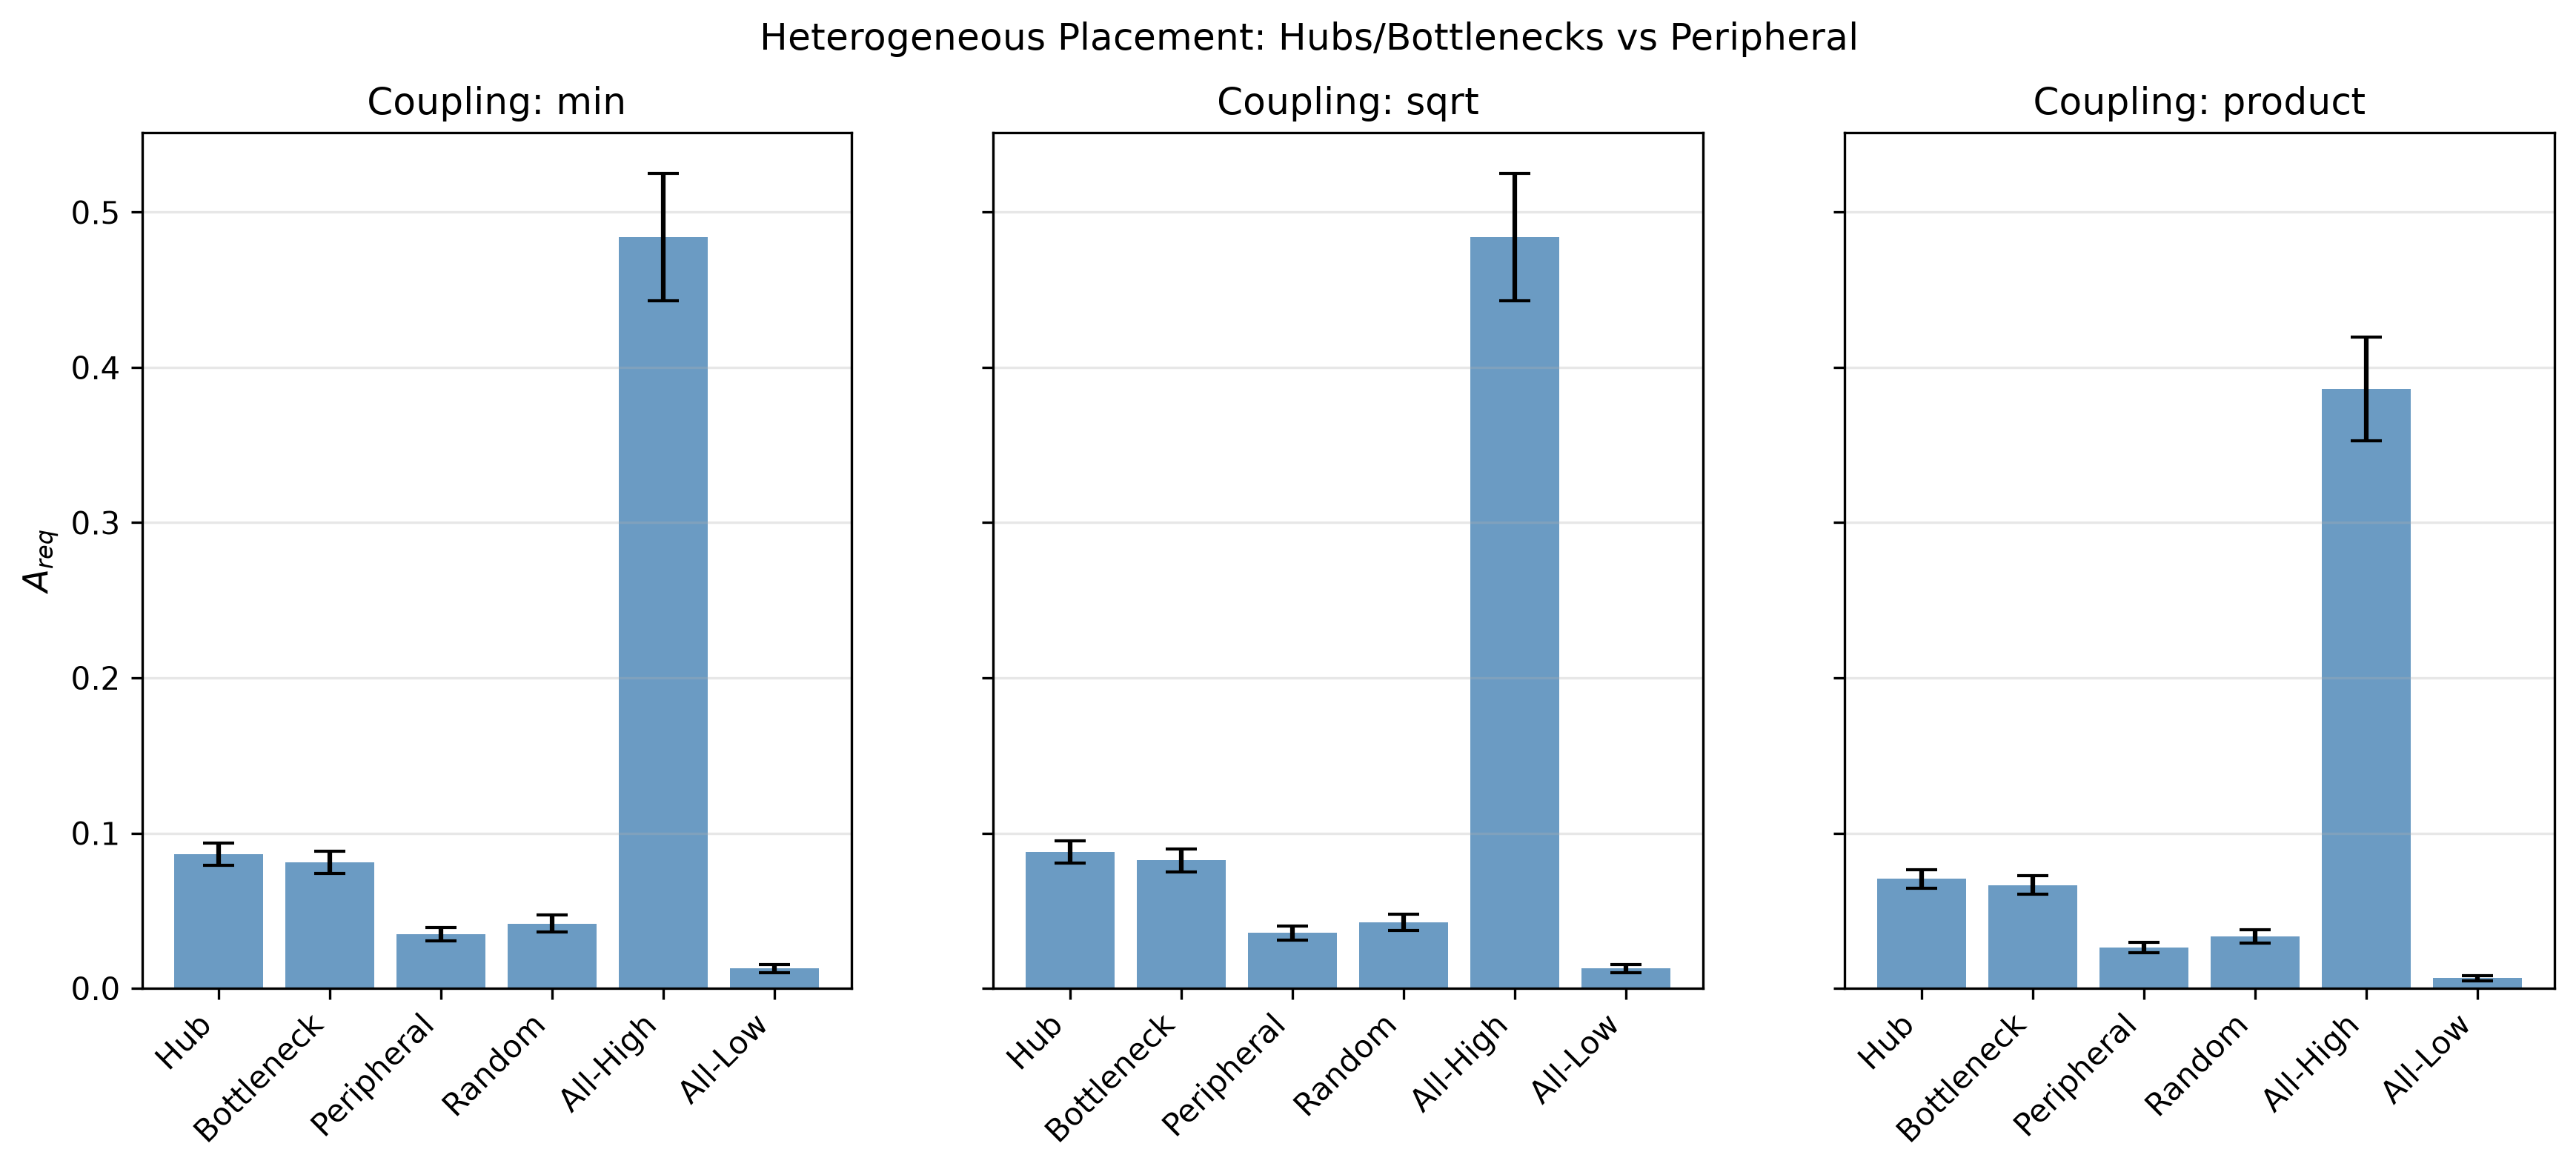
\includegraphics[width=0.98\textwidth]{figures/fig_heterogeneity_v05.png}
\caption{Heterogeneous placement results across three coupling rules. Aggregated across the tested configurations, hub and bottleneck placement outperform peripheral placement, although the per-topology ranking is not universal.}
\label{fig:heterogeneity}
\end{figure*}

\subsection{Interface-Coupling Model Sensitivity}

The three coupling rules ($\min$, $\sqrt{\eta_i \eta_j}$, $\eta_i \eta_j$) are alternative model assumptions used to test sensitivity to the physical interface between heterogeneous memories at the two endpoints of a link. They produce different absolute performance levels but preserve the ranking of placement strategies. The $\min$ and $\sqrt{\cdot}$ rules produce similar absolute levels (within 2\%), while the product rule lowers absolute $A_{\rm req}$ by 18--25\% depending on strategy. These coupling rules are explicit modeling assumptions and are not native concepts in the external frameworks used in the cross-implementation study; they have not been independently validated. This confirms that heterogeneous-memory conclusions require explicit interface modeling.

\subsection{Gap Between Mixed and All-High Placement}

A notable finding is the large gap between any mixed placement and the all-high baseline: mixed strategies recover only 8--18\% of the all-high performance. This gap quantifies the cost of heterogeneous hardware and is a distinct result from the ranking of mixed strategies.

\FloatBarrier

\section{Global Sensitivity Analysis}\label{sec:sensitivity}

\subsection{Permutation Importance Cross-Check}

As an independent sensitivity cross-check, we compute permutation importance using a Random Forest surrogate trained on the 67{,}584 A08 samples. Permutation importance measures which variables the surrogate is most dependent on for its predictions; it does not directly measure causal physical importance. The surrogate's held-out $R^2$ and MAE are reported alongside the importance values to contextualize their reliability (Table~\ref{tab:rf_r2}).

\begin{table}[htbp]
\centering
\caption{Random Forest surrogate performance on held-out data (20\% test split, 200 trees). Per-topology $R^2$ is high; the lower overall $R^2$ reflects topology as a major driver not included as a feature.}
\label{tab:rf_r2}
\begin{tabular}{lrrr}
\toprule
Topology & $n$ & $R^2$ & MAE \\
\midrule
All (pooled) & 67{,}584 & 0.423 & 0.142 \\
Chain & 22{,}528 & 0.944 & 0.015 \\
Star & 22{,}528 & 0.972 & 0.019 \\
RGG & 22{,}528 & 0.974 & 0.023 \\
\bottomrule
\end{tabular}
\end{table}

The per-topology $R^2$ values (0.94--0.97) indicate that the surrogate captures the within-topology input--output mapping well, so the permutation importance values are reliable as \emph{predictive} associations. The pooled $R^2 = 0.42$ confirms that topology is a major driver of performance that is not captured by the 10 varied parameters alone. Table~\ref{tab:sens_params} lists the parameter ranges, and Figure~\ref{fig:sensitivity} shows the permutation importance by topology.

\begin{table}[htbp]
\centering
\caption{Parameter ranges for the sensitivity analysis. Log-scaled parameters are sampled uniformly in log-space.}
\label{tab:sens_params}
\begin{tabular}{llll}
\toprule
Parameter & Min & Max & Scale \\
\midrule
$\eta_r$ (retrieval eff.) & 0.30 & 0.99 & linear \\
$F_{ro}$ (readout fid.) & 0.90 & 0.999 & linear \\
$T_2$ & 0.001 s & 10 s & log \\
$p_{\rm gen}$ & 0.001 & 0.05 & log \\
$t_{\rm attempt}$ & $10^{-5}$ s & $10^{-2}$ s & log \\
$m$ (memory budget) & 1 & 8 & discrete \\
$\lambda$ (arrival rate) & 1.0 & 100.0 & log \\
noise scale & 0.1 & 10.0 & linear \\
$N$ (network size) & 10 & 50 & discrete \\
$F_{\rm initial}$ & 0.85 & 0.99 & linear \\
\bottomrule
\end{tabular}
\end{table}

\begin{figure*}[t]
\centering
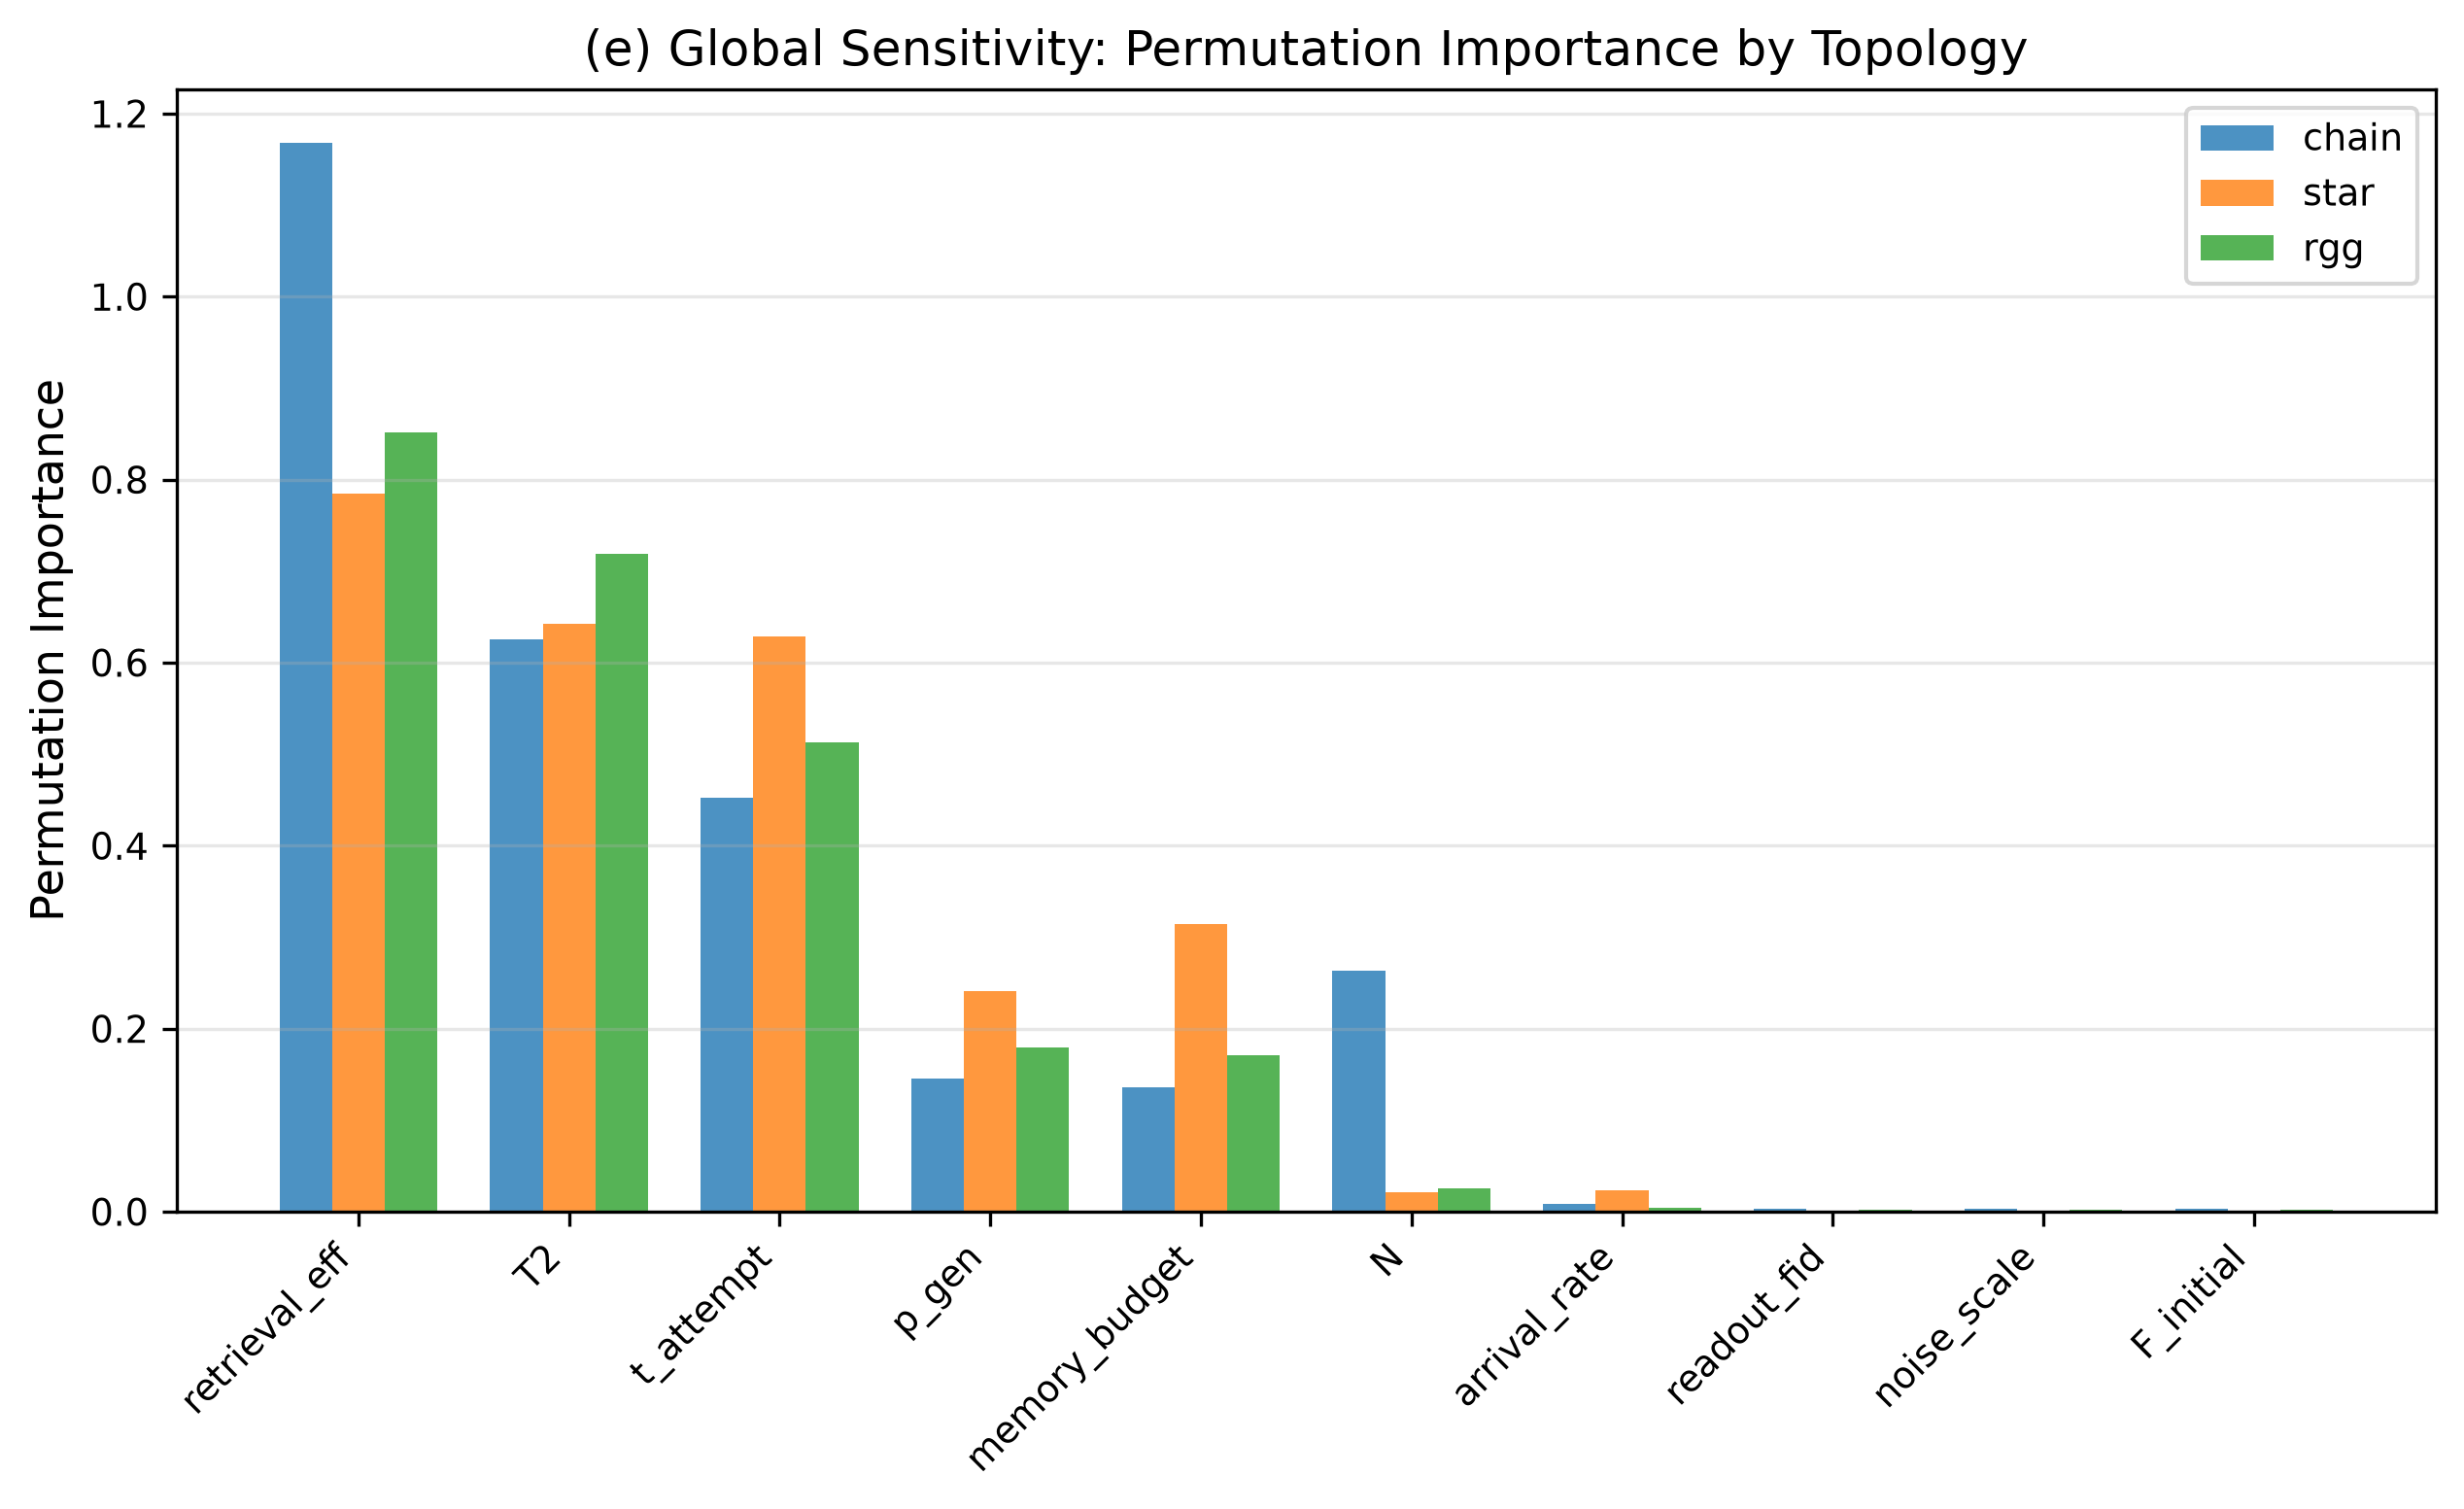
\includegraphics[width=0.85\textwidth]{figures/fig_a8_sensitivity.png}
\caption{Permutation importance by topology. Retrieval efficiency is consistently the most important parameter across all three topologies, followed by $T_2$ and $t_{\rm attempt}$.}
\label{fig:sensitivity}
\end{figure*}

\textbf{Result:} Retrieval efficiency is consistently ranked as the most informative predictor by the Random Forest surrogate across all three tested topologies (permutation importance 0.78--1.15), followed by $T_2$ (0.61--0.67) and $t_{\rm attempt}$ (0.40--0.59). The qualitative surrogate ranking is reproducible. The qualitative ranking is reproducible across topologies.

\textbf{Caveat:} Retrieval efficiency $\eta_r$ enters the success probability multiplicatively, so its high importance is partly structural rather than purely physical. The importance of $\eta_r$ should be interpreted as ``most informative for the surrogate's predictions,'' not as ``causally dominant in the physical system.'' The broad range of $\eta_r$ (0.30--0.99) also contributes to its high ranking; a narrower range would likely reduce its importance. The feature-importance ordering has not yet been evaluated across independent simulation models.

\textbf{Why $T_2$ ranks high in the surrogate.} The permutation-importance analysis ranks $T_2$ as the second-most informative predictor (0.61--0.67). In the atlas dataset, $T_2$ and $\tau_r$ are perfectly collinear across the six memory families (Spearman $\rho = 1.0$). The surrogate therefore uses $T_2$ as a proxy for $\tau_r$; permuting $T_2$ destroys the proxy and degrades predictions. The surrogate's high ranking for $T_2$ is therefore a consequence of collinearity in the training data, not necessarily of independent physical causation. The three metrics---$A_{\rm req}$ (delivery without fidelity), $A_{\rm qual}$ (delivery with fidelity threshold), and fidelity at delivery---are affected differently: $T_2$ affects fidelity and $A_{\rm qual}$ through decoherence; $\tau_r$ affects all three through retrieval decay. A surrogate trained on $A_{\rm qual}$ or fidelity would rank $T_2$ highly for a direct physical reason; a surrogate trained on $A_{\rm req}$ may rank $T_2$ highly because it proxies for $\tau_r$.

\FloatBarrier

\section{Design Implications}

\begin{enumerate}[leftmargin=2em]
\item \textbf{The $\chi_r$ descriptor provides a physical timescale interpretation.} The coincidence-window parameter $\chi_r = \tau_r\, p_{\rm gen} / t_{\rm attempt}$ (where $\tau_r$ is the retrieval decay time) separates queue-limited ($\chi_r \gg 1$) from coincidence-limited ($\chi_r \ll 1$) regimes and is consistent with the observed per-family $m_c$ distribution. No predictive accuracy or invariance rate is asserted for $\chi_r$ in this revision. For network planning, $\chi_r$ can be computed from device parameters as a physical descriptor, but it does not establish a network memory-sizing law.

\item \textbf{Memory selection cannot be reduced to coherence time alone.} Retrieval efficiency, coherence, and waiting-time-induced decoherence interact; retrieval efficiency and coherence time rank highly in the tested surrogate analyses, while memory-profile choice produces large performance differences. This is a structural conclusion; the specific importance values are model-specific estimates.

\item \textbf{Retrieval efficiency, coherence, and waiting time interact.} The cross-implementation check reproduced the ordering of the evaluated memory profiles under the fidelity-qualified metric, confirming that the family ordering is a structural finding within the tested model class.

\item \textbf{Network topology changes the value of a given memory resource.} The confirmatory subset exhibits a topology effect (RGG mean $A_{\rm req}=0.233$ vs chain mean $0.082$), though this comparison is confounded with path length and total memory (topologies with more nodes receive more total memory under the per-node budget definition). The RGG $>$ star $>$ chain ordering was reproduced in the cross-implementation check. The tested scalar scaling hypotheses remain topology-dependent, so mean path-length corrections alone are insufficient to collapse the observed variation.

\item \textbf{Memory overprovisioning thresholds are regime-specific.} A single $m_c$ value does not describe the tested configurations; capacity planning must account for memory profile, topology, and offered load. The $m_c$ values reported here are model-specific quantitative estimates of the WestQuant simulation; the structural conclusion that $m_c$ is regime-dependent is robust.

\item \textbf{High-quality resources should preferentially occupy structurally important nodes under the tested placement model.} Assigning high-quality memories to hubs or traffic-bottleneck nodes outperforms peripheral placement, and the strategy ordering is unchanged across the three coupling rules. This is a structural conclusion; the placement result has not yet been cross-implemented.

\item \textbf{Interface assumptions can materially alter absolute performance.} Coupling-rule assumptions affect absolute performance by 18--25\%. The interface-coupling rules are explicit modeling assumptions and have not been independently validated. Heterogeneous-memory conclusions require explicit interface modeling.
\end{enumerate}

The representative memory profiles used here are parameter bundles, not complete realized hardware stacks; the design messages above are qualitative rather than device-certification-level.

\FloatBarrier

\section{Limitations}

\begin{enumerate}[leftmargin=2em]
\item \textbf{Cross-implementation rather than full native-protocol validation.} In addition to analytical component checks, selected conclusions were tested through harmonized implementations executed on SeQUeNCe and SimQN event frameworks. The two external adapters share a common harmonized model and therefore do not constitute two independent physical-model replications. Native SeQUeNCe/SimQN protocols, NetSquid, and QuISP were not included.

\item \textbf{Absolute-value model dependence.} Cross-implementation comparisons indicate that absolute performance values are more implementation-sensitive than the tested topology and memory-profile orderings.

\item \textbf{Critical memory capacity.} Numerical critical-memory thresholds have not yet been cross-validated using the full $m=\{1,2,4,8,16,32,64\}$ sweep.

\item \textbf{Heterogeneous placement.} The heterogeneous placement result has not yet been cross-implemented.

\item \textbf{Interface-coupling rules.} The interface-coupling rules are explicit modeling assumptions and have not been independently validated.

\item \textbf{Metric semantics.} Completion and latency metrics are sensitive to queueing, censoring, and timing definitions; future native-protocol comparisons must harmonize these definitions before quantitative comparison.

\item \textbf{Scalar collapse.} The scalar-collapse result has not yet been independently cross-implemented.

\item \textbf{Sobol bootstrap bug.} The Saltelli bootstrap confidence intervals were found to be unreliable due to a structural resampling bug (resampling individual rows instead of Saltelli blocks). Sobol indices are therefore not reported as quantitative results; fixing the bootstrap and rerunning is future work. We rely on permutation importance for qualitative ranking.

\item \textbf{Representative memory parameters.} Memory families use representative parameter bundles, not complete hardware-stack comparisons. Real devices have additional noise sources.

\item \textbf{Uniform traffic in main atlas.} Most atlas experiments use uniform traffic. Traffic-matrix support exists but is not exercised in the main atlas.

\item \textbf{No purification or multiplexing.} The simulator does not model entanglement purification or spatial multiplexing.

\item \textbf{Limited network sizes.} Experiments cover $N \in [10, 50]$. Scaling to $N \geq 100$ is future work.

\item \textbf{Routing policy.} We use shortest-hop routing. Other policies may change conclusions.

\item \textbf{No dynamic traffic.} Traffic is Poisson with fixed rate. Time-varying traffic belongs to future work.

\item \textbf{Atlas and confirmatory grid completeness.} The atlas design contains 9{,}720 nominal cells; 9{,}360 completed runs are retained (360 missing, 3.7\%). The confirmatory grid contains 9{,}000 cells; 8{,}730 completed simulations are retained (270 missing, 3.0\%). Missing cells arise from disconnected random-geometric graphs and simulation failures and are not imputed.

\item \textbf{Topology fairness: per-node vs total-memory confound.} Because $m$ is defined as the per-node budget, topologies with more nodes receive more total memory. Cross-topology comparisons therefore conflate topology structure with total resource allocation. A fixed-total-memory design would be needed to isolate the pure topology effect.

\item \textbf{Topology-dependent exclusion of no-path requests.} The metric $A_{\rm req}$ excludes no-path requests from the denominator. Because the fraction of no-path requests depends on topology (e.g., disconnected RGGs produce more no-path requests than fully connected chains), the effective denominator varies across topologies, potentially biasing cross-topology comparisons.

\item \textbf{Seed and request quantization.} The atlas uses 5 seeds and 100 requests per simulation. With only 100 requests, $A_{\rm req}$ is quantized to multiples of $1/100$, limiting resolution for small differences. The confirmatory dataset uses 20 seeds, which reduces but does not eliminate this quantization effect.

\item \textbf{$m_c$ relative to observed maximum.} The threshold $m_c$ is defined relative to $A_{\max}^{\rm obs}$, the maximum on the observed budget grid, not an asymptotic limit. If the budget-response curve has not plateaued, $m_c$ underestimates the budget needed to reach a fixed fraction of the true asymptotic performance. This is a fundamental limitation of grid-based threshold estimation.

\item \textbf{RGG disconnection selection bias.} Disconnected random-geometric graphs are excluded from the analysis (contributing to the 360 missing atlas cells and 270 missing confirmatory cells). This creates a selection bias: the surviving RGG instances are those with sufficient edge density to remain connected, which may overstate RGG performance relative to a random draw from the RGG ensemble.

\item \textbf{Readout-model discrepancy.} The frozen datasets were generated with a multiplicative readout model ($F_{\rm out} = F_{ro} \cdot F$), while the current codebase uses a depolarizing model ($F_{\rm out} = F_{ro} \cdot F + (1-F_{ro}) \cdot 0.25$). The difference is 1--2.5\% in fidelity (systematic: the depolarizing model yields higher fidelity than the multiplicative model for $F_{ro} < 1$ and $F > 0.25$). This does not affect the retrieval-window descriptor $\chi_r$ because $\chi_r$ depends on $\tau_r$ and generation parameters, not readout. Regenerating the frozen datasets with the depolarizing model is future work.

\item \textbf{Run length at high traffic.} With $n_{\rm requests} = 100$ and $\lambda = 50$, the observation window is approximately 2~s, which may not reach full stationarity for queueing dynamics at high load. Results at $\lambda = 50$ should be interpreted with this caveat.
\end{enumerate}

\FloatBarrier

\section{Conclusion}

Memory capacity requirements in the tested quantum-network model depend on memory profile, topology, and traffic. The finite-grid threshold reaches the upper tested budget in 35.5\% of the reported regimes, and it must be distinguished from an asymptotic saturation capacity. The tested scalar reductions leave substantial topology-dependent variation. Correctly using retrieval decay time in $\chi_r$ provides a physical timescale descriptor but does not establish a universal sizing law. Heterogeneous placement favors hubs and betweenness-based nodes in aggregate, while topology-specific exceptions and coupling-dependent absolute performance limit generalization. These findings support explicit, model-specific capacity planning and targeted validation of the decisions to be deployed.

\section*{Data Availability and Reproducibility}

The manuscript and a repository scaffold are prepared for a dedicated public reproducibility release. The raw simulation datasets, frozen simulator, dependency lockfile, complete seed/configuration ledger, and figure-generation scripts have not yet been deposited in that release. The development repository is private. This revision therefore does not claim that the empirical results can already be reproduced from a public archive. A public release URL, commit identifier, checksums, and archival DOI should identify the completed deposit before submission.

\section*{Relationship to Companion Work}

A companion methods manuscript, ``Assessing Decision Reliability in Discrete-Event Simulation: A Quantum-Network Case Study,'' studies stochastic decision stability, metric semantics, and model sensitivity. The present article focuses on memory-profile, capacity, topology, and placement results. Shared simulator infrastructure and overlapping validation results should be disclosed to both editors.

\section*{Competing Interests}

The author is the founder of Vesterlund Ventures and WestQuant Open. The simulator used in this study (WestQuant) was developed by the author. This creates a potential conflict of interest insofar as the simulator's design choices may influence the results. The cross-implementation robustness check (Sec.~\ref{sec:cross_impl}) partially mitigates this concern by testing whether selected conclusions survive an independent implementation pathway, but does not eliminate it. The author has no external funding to declare.

\section*{Author Contributions}

D.V. conceived the study, designed and implemented the simulator, ran all experiments, performed all analyses, and wrote the manuscript.

\section*{Funding}

This research received no external funding. Computational resources were provided by the author's personal hardware. No GPU or compute-cluster grants were used.

\section*{Acknowledgments}

The author acknowledges the use of open-source quantum-network simulation frameworks SeQUeNCe~\cite{wu2021sequence} and SimQN in the cross-implementation robustness check.

\textbf{AI-assisted tools.} AI-assisted tools (Anthropic Claude, OpenAI ChatGPT, and Cognition Devin) were used during the preparation of this work, including assistance with code generation, manuscript organization, and editorial revision. The author takes full responsibility for the work. During the preparation, several errors were introduced by the AI tools and caught by Claude acting as an external reviewer, including: (1) the original $\chi = T_2\, p_{\rm gen}/t_{\rm attempt}$ used the wrong lifetime parameter (corrected to $\chi_r = \tau_r\, p_{\rm gen}/t_{\rm attempt}$); (2) the $m=1$ failure was attributed to swap contention (corrected to slot contention after two-node testing); (3) predictive accuracy and invariance claims for $\chi_r$ were overstated and have been removed in this revision.

\begin{thebibliography}{39}

\bibitem{wehner2018quantum}
S.~Wehner, D.~Elkouss, and R.~Hanson,
Quantum internet: A vision for the road ahead,
\textit{Science} \textbf{362}, eaam9288 (2018).

\bibitem{razavi2009quantum}
M.~Razavi, M.~Piani, and N.~L{\"u}tkenhaus,
Quantum repeaters with imperfect memories: Cost and scalability,
\textit{Phys. Rev. A} \textbf{80}, 032301 (2009).

\bibitem{sangouard2011quantum}
N.~Sangouard, C.~Simon, H.~de~Riedmatten, and N.~Gisin,
Quantum repeaters based on atomic ensembles and linear optics,
\textit{Rev. Mod. Phys.} \textbf{83}, 33 (2011).

\bibitem{kamin2023exact}
L.~Kamin, E.~Shchukin, F.~Schmidt, and P.~van Loock,
Exact rate analysis for quantum repeaters with imperfect memories and entanglement swapping as soon as possible,
\textit{Phys. Rev. Research} \textbf{5}, 023086 (2023).

\bibitem{chehimi2023scaling}
M.~Chehimi, S.~Pouryousef, N.~K.~Panigrahy, D.~Towsley, and W.~Saad,
Scaling limits of quantum repeater networks,
arXiv:2305.08696 (2023).

\bibitem{wu2021sequence}
X.~Wu, A.~Kolar, J.~Chung, D.~Jin, T.~Zhong, R.~Kettimuthu, and M.~Suchara,
SeQUeNCe: A customizable discrete-event simulator of quantum networks,
\textit{Quantum Sci. Technol.} \textbf{6}, 045022 (2021).

\bibitem{coopmans2021netsquid}
T.~Coopmans, R.~Knegjens, A.~Dahlberg, D.~Ferrari, J.~Rabbie, and S.~Wehner,
NetSquid, a network simulator for quantum information using discrete events,
\textit{Commun. Phys.} \textbf{4}, 164 (2021).

\bibitem{satoh2022quisp}
R.~Satoh, M.~Hajdu{\v{s}}ek, N.~Benchasattabuse, S.~Suzuki, R.~Van~Meter, and H.~Takesue,
QuISP: A quantum internet simulation package,
in \textit{2022 IEEE Int. Conf. on Quantum Computing and Engineering (QCE)}, pp.~353--364 (2022).

\bibitem{vittal2025cross}
J.~Chung, M.~Hajdu\v{s}ek, N.~Benchasattabuse, A.~Kolar, A.~Singal, K.~S.~Soon, K.~Teramoto, A.~Zang, R.~Kettimuthu, and R.~Van~Meter,
Cross-validating quantum network simulators,
arXiv:2504.01290 (2025).

\bibitem{sharma2024heterogeneous}
K.~S.~Soon, N.~Benchasattabuse, M.~Hajdu\v{s}ek, K.~Teramoto, S.~Nagayama, and R.~Van~Meter,
Performance of quantum networks using heterogeneous link architectures,
in \textit{2024 IEEE Int. Conf. on Quantum Computing and Engineering (QCE)}, pp.~1914--1923 (2024), arXiv:2405.09862.

\bibitem{van2025hybrid}
S.~Sun, D.~Bhatti, S.~Gao, D.~Elkouss, and H.~Takahashi,
Hybrid quantum repeater chains with atom-based quantum processing units and quantum memory multiplexers,
arXiv:2512.21655 (2025).

\bibitem{liu2025hybrid}
P.~Cussenot, B.~Grivet, B.~P.~Lanyon, T.~E.~Northup, H.~de~Riedmatten, A.~S.~S{\o}rensen, and N.~Sangouard,
Uniting quantum processing nodes of cavity-coupled ions with rare-earth quantum repeaters using single-photon pulse shaping based on atomic frequency comb,
\textit{Phys. Rev. Lett.} \textbf{135}, 240803 (2025), arXiv:2501.18704.

\bibitem{alhejji2026topology}
K.~Ooi, G.~Sutcliffe, and M.~Beghelli,
Impact of topology on multipartite entanglement distribution protocols in quantum networks,
\textit{J. Opt. Commun. Netw.} \textbf{18}, 1054 (2026).

\bibitem{ozaydin2025multiring}
M.~Ozaydin et al.,
Optimal entanglement distribution within a multi-ring topology,
\textit{Sci. Rep.} (2025).

\bibitem{amin2023capacity}
G.~Vardoyan, E.~van~Milligen, S.~Guha, S.~Wehner, and D.~Towsley,
On the bipartite entanglement capacity of quantum networks,
\textit{IEEE Trans.\ Quantum Eng.} \textbf{5}, 1 (2024), arXiv:2307.04477.

\bibitem{pouryousef2024resource}
S.~Pouryousef, H.~Shapourian, A.~Shabani, R.~Kompella, and D.~Towsley,
Resource placement for rate and fidelity maximization in quantum networks,
arXiv:2308.16264 (2024).

\bibitem{sripotchanart2024twostep}
R.~Sripotchanart, W.~Si, R.~N.~Calheiros, Q.~Cao, and T.~Qiu,
A two-step linear programming approach for repeater placement in large-scale quantum networks,
\textit{Comput. Netw.} \textbf{254}, 110795 (2024).

\bibitem{islam2023scalable}
T.~Islam and E.~Arslan,
Scalable quantum repeater deployment modeling,
arXiv:2305.09855 (2023).

\bibitem{pirandola2019endtoend}
S.~Pirandola,
End-to-end capacities of a quantum communication network,
\textit{Commun. Phys.} \textbf{2}, 51 (2019).

\bibitem{takeoka2016rateloss}
M.~Takeoka, S.~Guha, and M.~M.~Wilde,
Fundamental rate-loss tradeoff for optical quantum communication,
\textit{Nat. Commun.} \textbf{7}, 13523 (2016).

\bibitem{vardoyan2021maxweight}
T.~Vasantam and D.~Towsley,
Stability analysis of a quantum network with max-weight scheduling,
arXiv:2106.00831 (2021).

\bibitem{langer2005long}
C.~Langer, R.~Ozeri, J.~D.~Jost, J.~Chiaverini, B.~DeMarco, A.~Ben-Kish, R.~B.~Blakestad, J.~Britton, D.~B.~Hume, W.~M.~Itano, D.~Leibfried, R.~Reichle, T.~Rosenband, T.~Schaetz, P.~O.~Schmidt, and D.~J.~Wineland,
Long-lived qubit memory using atomic ions,
\textit{Phys. Rev. Lett.} \textbf{95}, 060502 (2005).

\bibitem{wang2014high}
T.~P.~Harty, D.~T.~C.~Allcock, C.~J.~Ballance, L.~Guidoni, H.~A.~Janacek, N.~M.~Linke, D.~N.~Stacey, and D.~M.~Lucas,
High-fidelity preparation, gates, memory, and readout of a trapped-ion quantum bit,
\textit{Phys. Rev. Lett.} \textbf{113}, 220501 (2014).

\bibitem{wang2024fine}
Y.~Wang et al.,
Coherent control of the fine-structure qubit in a single alkaline-earth atom,
\textit{Phys. Rev. Lett.} \textbf{132}, 150606 (2024).

\bibitem{hosseini2006gem}
M.~Hosseini, B.~M.~Sparkes, G.~Campbell, P.~K.~Lam, and B.~C.~Buchler,
High efficiency coherent optical memory with warm rubidium vapour,
\textit{Nat. Commun.} \textbf{2}, 174 (2011).

\bibitem{wang2018eit}
Y.-F.~Hsiao, P.-J.~Tsai, H.-S.~Chen, S.-X.~Lin, C.-C.~Hung, C.-H.~Lee, Y.-H.~Chen, Y.-F.~Chen, I.~A.~Yu, and Y.-C.~Chen,
Highly efficient coherent optical memory based on electromagnetically induced transparency,
\textit{Phys. Rev. Lett.} \textbf{120}, 183602 (2018).

\bibitem{balasubramanian2009ultralong}
G.~Balasubramanian et al.,
Ultralong spin coherence time in isotopically engineered diamond,
\textit{Nat. Mater.} \textbf{8}, 383 (2009).

\bibitem{steiner2010universal}
M.~Steiner, P.~Neumann, J.~Beck, F.~Jelezko, and J.~Wrachtrup,
Universal enhancement of the optical readout fidelity of single electron spins at nitrogen-vacancy centers in diamond,
\textit{Phys. Rev. B} \textbf{81}, 035205 (2010).

\bibitem{bradley2022robust}
C.~E.~Bradley et al.,
Robust quantum-network memory based on spin qubits in isotopically engineered diamond,
\textit{npj Quantum Inf.} \textbf{8}, 122 (2022).

\bibitem{maurer2012room}
P.~C.~Maurer, G.~Kucsko, C.~Latta, L.~Jiang, N.~Y.~Yao, S.~D.~Bennett, F.~Pastawski, D.~Hunger, N.~Chisholm, M.~Markham, D.~J.~Twitchen, J.~I.~Cirac, and M.~D.~Lukin,
Room-temperature quantum bit memory exceeding one second,
\textit{Science} \textbf{336}, 1283 (2012).

\bibitem{rielandner2021storage}
A.~Ortu, A.~Holz\"apfel, J.~Etesse, and M.~Afzelius,
Storage of photonic time-bin qubits for up to 20~ms in a rare-earth doped crystal,
\textit{npj Quantum Inf.} \textbf{8}, 29 (2022).

\bibitem{laplane2017multimode}
C.~Laplane, P.~Jobez, J.~Etesse, N.~Gisin, and M.~Afzelius,
Multimode and long-lived quantum correlations between photons and spins in a crystal,
\textit{Phys. Rev. Lett.} \textbf{118}, 210501 (2017).

\bibitem{reagor2016quantum}
M.~Reagor et al.,
Quantum memory with millisecond coherence in circuit QED,
\textit{Phys. Rev. B} \textbf{94}, 014506 (2016).

\bibitem{sm}
See Supplemental Material at \url{https://github.com/VesterlundCoder/quantum-network} (supplemental material) for full parameter provenance (Table~S1), complete $m_c$ tables (Table~S2), cross-implementation validation appendix (Table~S6), and nonlinear scalar-collapse details (Table~S7). Sobol sensitivity tables (formerly S3--S5) have been removed due to the bootstrap bug described in Sec.~\ref{sec:sensitivity}.

\end{thebibliography}

\end{document}
